\documentclass[a4paper,12pt]{article}
\usepackage[russian]{babel}
\usepackage[T2A]{fontenc}
\usepackage[utf8]{inputenc}
\usepackage[russian]{babel}
\usepackage{geometry}
\usepackage{amsmath}
\usepackage{graphicx}
\usepackage{cancel}
\usepackage{float} 
\usepackage{xcolor}
\usepackage{listings}
\usepackage{hyperref}
\usepackage{array}
\usepackage{caption}
\usepackage{booktabs}
\usepackage{amssymb}
\usepackage{subcaption}
\usepackage{caption}
\captionsetup[figure]{name=Рисунок}
\captionsetup[table]{name=Таблица}
\usepackage{pgfplots}
\pgfplotsset{compat=1.18}
\usetikzlibrary{arrows.meta}
\usepackage{capt-of}
\usepackage{multirow}
\usepackage[siunitx]{circuitikz}
\usepackage[bottom]{footmisc}
\usepackage{tcolorbox}
\usepackage{nicematrix}
\usepackage{tikz}
\usepackage{amssymb}

\usetikzlibrary{arrows.meta, matrix}
\lstset{
	language=Matlab,
	basicstyle=\ttfamily\small,
	keywordstyle=\color{blue}\bfseries,
	commentstyle=\color{gray}\itshape,
	stringstyle=\color{red},
	numberstyle=\tiny\color{gray},
	numbers=left,
	stepnumber=1,
	numbersep=8pt,
	backgroundcolor=\color{white},
	frame=single,
	breaklines=true,
	breakatwhitespace=true,
	tabsize=4,
	showspaces=false,
	showstringspaces=false,
	captionpos=b,
	escapeinside={\%*}{*)},
}
\geometry{left=1.5cm, right=2cm, bottom=2cm, top=2cm}

\begin{document}

\begin{titlepage}
	\centering
	
	\vspace*{0.5cm}
	{\small
		Министерство науки и высшего образования Российской Федерации\\[2pt]
		Федеральное государственное автономное образовательное учреждение\\
		высшего образования\\[2pt]
		\textbf{«Национальный исследовательский университет ИТМО»}\\
	}
	
	\vspace{0.8cm}
	\hrule height 0.8pt
	\vspace{0.3cm}
	
	{\large Факультет систем управления и робототехники}
	
	\vspace{0.3cm}
	\hrule height 0.4pt
	\vspace{2.5cm}
	
	{\Huge\bfseries ОТЧЁТ}\\[0.4cm]
	{\LARGE\bfseries о лабораторной работе}\\[0.8cm]
	
	\begin{tcolorbox}[
			colback=gray!4,
			colframe=gray!10,
			boxrule=0.8pt,
			arc=4pt,
			left=12pt, right=12pt, top=8pt, bottom=8pt
		]
		\centering
		{\large По дисциплине:\\[4pt]}
		{\large\bfseries «Теория автоматического управления»}\\[10pt]
		{\large Тема:\\[4pt]}
		{\large\bfseries «Модальные регуляторы и наблюдатели»} \\[10pt]
		{\large Поток: 1.1.3 \( \) Вариант: 25}
	\end{tcolorbox}
	
	\vspace{3cm}
	
	\begin{minipage}{0.45\textwidth}
		\raggedright
		{\large\bfseries Студент:}\\[4pt]
		Охрименко Е.\,Д.\\
	\end{minipage}
	\hfill
	\begin{minipage}{0.45\textwidth}
		\raggedleft
		{\large\bfseries Преподаватель:}\\[4pt]
		Пашенко А.\,В.\\
	\end{minipage}
	
	\vfill
	\vspace{0.4cm}
	{\large Санкт-Петербург, 2026}
\end{titlepage}
\newpage
\tableofcontents



\newpage
\section{Модальный регулятор}
\label{sec:task1}

В соответствии с вариантом рассмотрю систему:

\[
\dot{x} = 
\begin{bmatrix}
	8 & 1 & 11 \\
	4 & 0 & 4 \\
	-4 & -3 & -7 \\
\end{bmatrix} x + 
\begin{bmatrix}
	-1 \\ -3 \\ 3
\end{bmatrix} u
\]

Требуется:

\begin{itemize}
	\item Найти собственные числа матрицы $A$, определить управляемость и стабилизируемость системы.
	\item Для каждого достижимого спектра:
	\begin{itemize}
		\item Синтезировать матрицу регулятора $K$ тремя методами: уравнение Сильвестра, метод модального управления, формула Аккермана\(/\)Басса-Гура.
		\item Проверить спектр матрицы замкнутой системы $(A + BK)$.
		\item Выполнить моделирование, построить графики $u(t)$ и $x(t)$ при $x(0) = \begin{bmatrix} 1 & 1 & 1 \end{bmatrix}^\top$.
	\end{itemize}
	\item Сопоставить результаты для различных спектров, выявить преимущества и недостатки каждого.
\end{itemize}

\hrule \newpage

\subsection{Управляемость собственных чисел матрицы \(A\)}

Для начала найду собственные числа матрицы $A$, решив характеристическое уравнение $\det(\lambda I - A) = 0$:

\[
\det(\lambda I - A) =
\det\begin{bmatrix}
	\lambda - 8 & -1 & -11 \\
	-4 & \lambda & -4 \\
	4 & 3 & \lambda + 7
\end{bmatrix} = 0
\]

Получаю характеристическое уравнение и следующие собственные числа:
\[
\lambda^3 - \lambda^2 - 4\lambda + 24 = 0
\qquad \Longrightarrow \qquad
\lambda_1 = -3, \quad \lambda_{2,3} = 2 \pm 2i
\]

Для оценки управляемости каждого собственного числа, построю Жорданову вещественную форму (листинг~\ref{lst:jordan1}). Тогда система в Жордановом базисе будет иметь вид:

\[
\dot{\hat{x}} = 
\begin{bNiceMatrix}[create-medium-nodes, left-margin=4pt, right-margin=4pt]
	-3 & 0 & 0 \\
	0 & 2 & -2 \\
	0 & 2 & 2 \\
	\CodeAfter
	\tikz \draw[red!80!black, rounded corners=2pt, line width=0.7pt, opacity=0.4] 
	([xshift=-2pt, yshift=2pt]1-1-medium.north west) rectangle 
	([xshift=2pt, yshift=-2pt]1-1-medium.south east);
	\tikz \draw[green!40!black, rounded corners=4pt, line width=0.7pt, opacity=0.4] 
	([xshift=-2pt, yshift=2pt]2-2-medium.north west) rectangle 
	([xshift=2pt, yshift=-2pt]3-3-medium.south east);
\end{bNiceMatrix}
\hat{x}  + 
\begin{bNiceMatrix}[create-medium-nodes, left-margin=4pt, right-margin=4pt]
	0 \\ 2.12 \\ 4.95 \\
	\CodeAfter
	\tikz \draw[red!80!black, rounded corners=2pt, line width=0.7pt, opacity=0.4]
	([xshift=-2pt, yshift=2pt]1-1-medium.north west) rectangle 
	([xshift=2pt, yshift=-2pt]1-1-medium.south east);
	\tikz \draw[green!40!black, rounded corners=4pt, line width=0.7pt, opacity=0.4]
	([xshift=-2pt, yshift=2pt]2-1-medium.north west) rectangle 
	([xshift=2pt, yshift=-2pt]3-1-medium.south east);
\end{bNiceMatrix}
u
\]

Собственное число \(\lambda_1 = -3\) неуправляемо, так как ему соответствует элемент \(0\) в матрице \(\hat{B}\). Собственные числа $\lambda_{2,3} = 2 \pm 2i$ управляемы, так как 
последняя строка соответствующего блока в матрице $\hat{B}$ ненулевая.

Получается, что система в целом не является полностью управляемой.

Неуправляемое собственное число \(\lambda_1 = -3\) лежит в левой комплексной полуплоскости, а значит система стабилизируема.

\subsection{Схема моделирования системы}

Построю модель замкнутой системы:

\[
\dot{x} = (A + BK)x
\]

\begin{figure}[H]
	\centering
	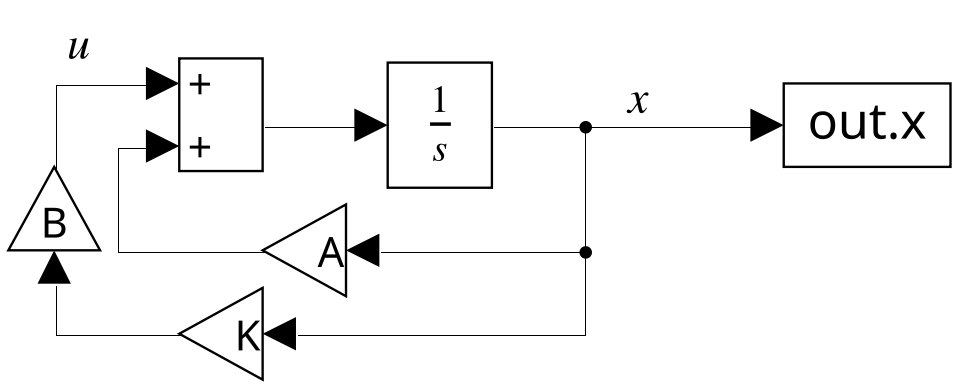
\includegraphics[width=0.6\textwidth]{../images/task1/model1.png}
	\caption{Структурная схема системы}
\end{figure}

\subsection{Достижимость спектров замкнутой системы}

Поскольку $\lambda_1 = -3$ неуправляемо, желаемый спектр достижим тогда и только тогда, когда он содержит $-3$. Рассмотрю предложенные спектры и сведу результаты в таблицу~\ref{tab:spectra}:

\begin{table}[H]
	\centering
	\caption{Анализ достижимости спектров}
	\label{tab:spectra}
	\begin{tabular}{ccc}
		\toprule
		№ & Спектр $\sigma(A + BK)$ & Достижимость \\
		\midrule
		1 & $\{-1,\ -1,\ -1\}$       & Нет \\
		2 & $\{-3,\ -3,\ -3\}$       & Да  \\
		3 & $\{-1,\ -10,\ -100\}$    & Нет \\
		4 & $\{-3,\ -30,\ -300\}$    & Да  \\
		5 & $\{-1,\ -1 \pm 3i\}$     & Нет \\
		6 & $\{-3,\ -3 \pm 9i\}$     & Да  \\
		\bottomrule
	\end{tabular}
\end{table}

Таким образом, достижимыми являются спектры №2, №4 и №6.

\subsection{Метод Сильвестра (спектр $\{-3,-3,-3\}$)}

Синтезирую регулятор с использованием матричного уравнения Сильвестра:
\[
\begin{cases}
	AP - P\Gamma = BY \\
	K = -YP^{-1}
\end{cases}
\]
где $\Gamma$ --- матрица с желаемым спектром, $Y$ --- вспомогательная матрица, пара $(Y,\ \Gamma)$ наблюдаема, $P$ --- решение уравнения.

Главное условие существования единственного решения $P$:
\[
\sigma(A) \cap \sigma(\Gamma) = \varnothing
\]
Условие не выполняется, так как спектр $\Gamma$ обязан содержать неуправляемое собственное число $\lambda_1 = -3$, чтобы желаемый спектр был достижим. Поэтому перейду в жорданов базис и отброшу строку и столбец, соответствующие $\lambda_1 = -3$:

\[
\begin{array}{c}
	\begin{array}{cc}
		\hat{A} =
		\begin{bNiceMatrix}[create-medium-nodes,left-margin=4pt,right-margin=4pt]
			-3 & 0 & 0 \\
			0 & 2 & -2 \\
			0 & 2 & 2 \\
			\CodeAfter
			\tikz \draw[red!80!black,line width=0.7pt,opacity=0.4]
			([xshift=-2pt]1-1-medium.west) -- ([xshift=2pt]1-3-medium.east);
			\tikz \draw[red!80!black,line width=0.7pt,opacity=0.4]
			([yshift=2pt]1-1-medium.north) -- ([yshift=-2pt]3-1-medium.south);
		\end{bNiceMatrix}
		&
		\hat{B} =
		\begin{bNiceMatrix}[create-medium-nodes,left-margin=4pt,right-margin=4pt]
			0 \\
			2.12 \\
			4.95 \\
			\CodeAfter
			\tikz \draw[red!80!black,line width=0.7pt,opacity=0.4]
			([xshift=2pt]1-1-medium.west) -- ([xshift=-2pt]1-1-medium.east);
		\end{bNiceMatrix}
	\end{array}
	\qquad \Longrightarrow \qquad
	\begin{array}{cc}
		\hat{A}_c =
		\begin{bmatrix}
			2 & -2 \\
			2 & 2
		\end{bmatrix}
		&
		\hat{B}_c =
		\begin{bmatrix}
			2.12 \\
			4.95
		\end{bmatrix}
	\end{array}
\end{array}
\]

Тогда уравнение Сильвестра для управляемой подсистемы:
\[
\begin{cases}
	\hat{A}_c P - P\Gamma = \hat{B}_c Y \\
	\hat K_c = -YP^{-1}
\end{cases}
\]
где $\hat{A}_c$, $\hat{B}_c$ --- усечённые матрицы в жордановом базисе.

Теперь выберу матрицы $\Gamma$ и $Y$. Поскольку желаемый спектр содержит кратное собственное число $-3$, матрицу $\Gamma$ удобно задать в виде жордановой клетки. Для обеспечения наблюдаемости пары $(Y,\Gamma)$ выберу матрицу $Y$ так, чтобы её первый элемент был ненулевым. Тогда:

\[
\Gamma =
\begin{bmatrix}
	-3 & 1 \\
	0 & -3
\end{bmatrix}
\qquad
Y =
\begin{bmatrix}
	1 & 2
\end{bmatrix}
\]

Запишу итоговое уравнение Сильвестра для управляемой подсистемы:

\[
\begin{cases}
	\begin{bmatrix}
		2 & -2 \\
		2 & 2
	\end{bmatrix}
	P
	-
	P
	\begin{bmatrix}
		-3 & 1 \\
		0 & -3
	\end{bmatrix}
	=
	\begin{bmatrix}
		2.12 \\
		4.95
	\end{bmatrix}
	\begin{bmatrix}
		1 & 2
	\end{bmatrix} \\[12pt]
	\hat K_c = -\,Y P^{-1}
\end{cases}
\]


Решу уравнение и найду матрицы \(P\) и \(\hat K_c\) (листинг~\ref{lst:silv1}). Получаю: 

\[
\begin{aligned}
	P &= \begin{bmatrix}
		0.70 & 1.58 \\
		0.70 & 1.49 \\
	\end{bmatrix} 
	\\[10pt]
	\hat K_c &= \begin{bmatrix}
		1.06 & -2.47
	\end{bmatrix}
\end{aligned}
\]


Приступлю к проверке корректности расчётов. Мне необходимо найти собственные числа матрицы замкнутой системы:

\[
\sigma(A + B K) \text{ --- ?}
\]

В это уравнение я не могу сразу подставить матрицу \(\hat K_c\), так как она имеет размерность \(1 \times 2\) и находится в жордановом базисе. Для того, чтобы размерности и базисы были одинаковы дополню ее нулем, соответствующим неуправляемому собственному числу и перейду из жорданового базиса в исходный (листинг~\ref{lst:origK11}):

\[
\hat K =
\begin{bmatrix}
	0 & 1.06 & -2.47
\end{bmatrix}
\qquad \Longrightarrow \qquad	
K =
\begin{bmatrix}
-3.5 & 1 & -3.5
\end{bmatrix}
\]

В результате подстановки матрицы обратной связи получаю матрицу замкнутой системы:

\[
A + BK =
\begin{bmatrix}
	11.5 & 0 & 14.5 \\
	14.5 & -3 & 14.5 \\
	-14.5 & 0 & -17.5
\end{bmatrix}
\]

Собственные числа матрицы (листинг~\ref{lst:eig1}):

\[
\sigma(A + BK) = \{-3, -3, -3\}
\]

Спектр совпадает с желаемым, значит все расчеты верны, матрица регулятора \(K\) синтезирована корректно. 

Выполню компьютерное моделирование замкнутой системы при начальных условиях 
$x(0) = \begin{bmatrix} 1 & 1 & 1 \end{bmatrix}^\top$. 
Результаты представлены на рисунках~\ref{fig:x11} и~\ref{fig:u11}:

\begin{figure}[H]
	\centering
	
\includegraphics[width=0.9\textwidth]{../images/task1/x1.pdf}
	\caption{Вектор состояния \(x(t)\)}
	\label{fig:x11}
\end{figure}

\begin{figure}[H]
	\centering
	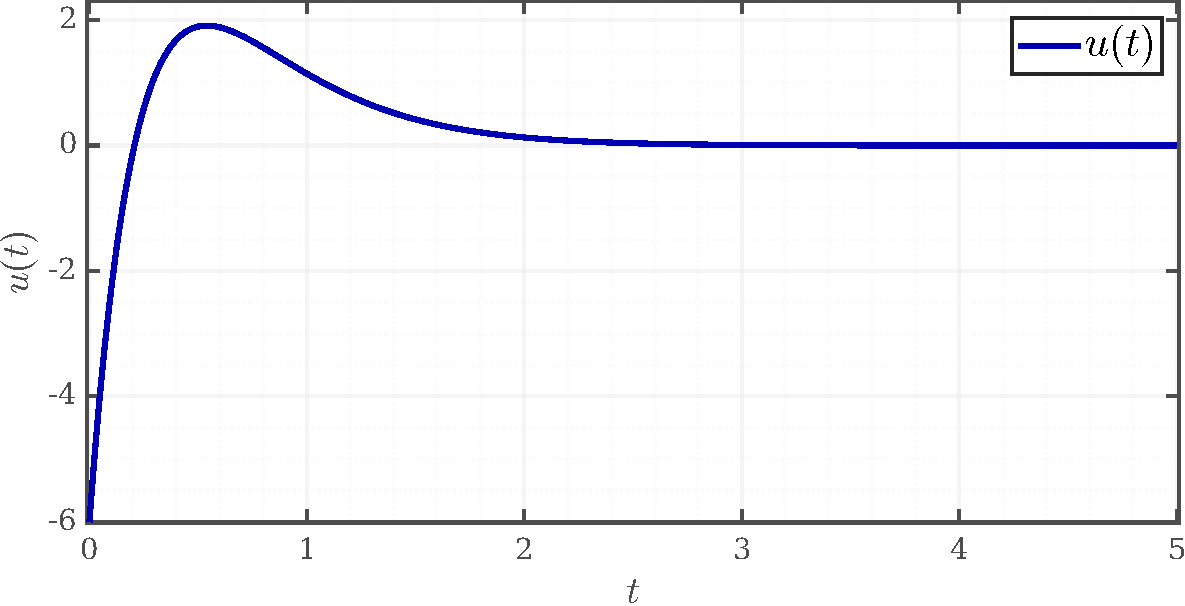
\includegraphics[width=0.9\textwidth]{../images/task1/u1.pdf}
	\caption{Управление \(u(t)\)}
	\label{fig:u11}
\end{figure}

Все компоненты вектора состояния асимптотически сходятся 
к нулю, что подтверждает корректность синтеза. Управление 
$u(t)$ также стремится к нулю.


\subsection{Метод модального управления (спектр $\{-3,\ -30,\ -300\}$)}

Синтезирую матрицу \(K\) при помощи модального управления. Возьму управляемую усеченную систему в жордановом базисе из прошлого подпункта:

\[
\dot{\hat x} = \begin{bmatrix}
	2 & -2 \\
	2 & 2
\end{bmatrix} \hat x + \begin{bmatrix}
	2.12 \\ 4.95
\end{bmatrix} u
\]

Выпишу желаемый характеристический полином спектра ($\lambda_1 = -3$ не учитываю, так как она подверглась усечению):

\[
(\lambda + 30)(\lambda + 300) = \lambda^2 + 330 \lambda + 9000
\]

Построю матрицу \(\Gamma\) в канонической управляемой форме:

\[
\Gamma = \begin{bmatrix}
	0 & 1 \\ -9000 & -330
\end{bmatrix}
\]

Теперь переведу систему в каноническую управляемую форму. Найду коэффициенты характеристического уравнения и определенным образом запишу их в матрицу \(A_{\text{упр},c}\):

\[
\operatorname{det}(\lambda I - \hat A_c) = \lambda^2 -4 \lambda + 8
\]

Тогда объект управления в канонической управляемой форме:

\[
\dot{x}_{\text{упр}} = 
\begin{bmatrix}
	0&1\\-8&4
\end{bmatrix} x_{\text{упр}} +
\begin{bmatrix}
	0 \\ 1
\end{bmatrix} u
\]

Замкнутая система в управляемом базисе имеет вид:
\[
\dot{x}_{\text{упр}} =
(A_{\text{упр},c} + B_{\text{упр},c} K_{\text{упр},c})\,x_{\text{упр}}
\qquad
K_{\text{упр},c} =
\begin{bmatrix}
	k_1 & k_2
\end{bmatrix}
\]

Подставляя матрицы \(A_{\text{упр},c}\) и \(B_{\text{упр},c}\), получаю:
\[
A_{\text{упр},c} + B_{\text{упр},c} K_{\text{упр},c}
=
\begin{bmatrix}
	0 & 1\\
	-8 & 4
\end{bmatrix}
+
\begin{bmatrix}
	0\\
	1
\end{bmatrix}
\begin{bmatrix}
	k_1 & k_2
\end{bmatrix}
=
\begin{bmatrix}
	0 & 1\\
	-8 + k_1 & 4 + k_2
\end{bmatrix}
\]

Согласно методу модального управления, матрица замкнутой системы должна совпадать с желаемой матрицей \(\Gamma\).

Приравнивая элементы последних строк, получаю систему уравнений:
\[
\begin{cases}
	-8 + k_1 = -9000 \\
	4 + k_2 = -330
\end{cases}
\qquad \Longrightarrow \qquad
\begin{cases}
	k_1 = -8992 \\
	k_2 = -334
\end{cases}
\qquad \Longrightarrow \qquad
K_{\text{упр},c} =
\begin{bmatrix}
	-8992 & -334
\end{bmatrix}
\]

Для перехода к жордановому базису использую преобразование:
\[
\hat K_c = K_{\text{упр},c} P_{\text{упр}}
\]
где \(P_{\text{упр}}\) --- матрица перехода в каноническую управляемую форму.

Матрица перехода в каноническую управляемую форму определяется через
матрицы управляемости исходной и канонической систем следующим образом:
\[
P_{\text{упр}} = U_c^* \hat U_c^{-1}
\]
где:

\[
\hat U_c =
\begin{bmatrix}
	\hat B_c & \hat A_c \hat B_c
\end{bmatrix}
\]
--- матрица управляемости исходной (усечённой) системы в текущем (жордановом) базисе,

\[
U_c^* =
\begin{bmatrix}
	B_{\text{упр},c} & A_{\text{упр},c} B_{\text{упр},c}
\end{bmatrix}
\]
--- матрица управляемости системы в канонической управляемой форме.

Проведу расчет \(P_{\text{упр}}\) в MATLAB (листинг~\ref{lst:P1}). В результате получаю:

\[
P_{\text{упр}} =
\begin{bmatrix}
	-0.0853 & 0.0366 \\
	-0.0975 & 0.2438
\end{bmatrix}
\]

Теперь с помощью этой матрицы найду \(\hat K_c\):

\[
\hat K_c =
\begin{bmatrix}
	799.96 & -410.32
\end{bmatrix}
\]

Приступлю к проверке корректности расчётов. Мне необходимо найти собственные числа матрицы замкнутой системы:

\[
\sigma(A + B K) \text{ --- ?}
\]

В это уравнение я не могу сразу подставить матрицу \(\hat K_c\), так как она имеет размерность \(1 \times 2\) и находится в жордановом базисе. Для того, чтобы размерности и базисы были одинаковы дополню ее нулем, соответствующим неуправляемому собственному числу и перейду из жорданового базиса в исходный (листинг~\ref{lst:origK11}, аналогично):

\[
\hat K =
\begin{bmatrix}
	0 & 799.96 & -410.32
\end{bmatrix}
\qquad \Longrightarrow \qquad	
K = \begin{bmatrix} -580.28 & -275.52 & -580.28 \end{bmatrix}
\]

В результате подстановки матрицы обратной связи получаю матрицу замкнутой системы:

\[
A + BK =
\begin{bmatrix}
	588.30 & 276.50 & 591.30 \\
	1744.80 & 826.60 & 1744.80 \\
	-1744.80 & -829.60 & -1747.80
\end{bmatrix}
\]

Собственные числа матрицы (листинг~\ref{lst:eig1}, аналогично):

\[
\sigma(A + BK) = \{-30, -300, -3\}
\]

Спектр совпадает с желаемым, значит все расчеты верны, матрица регулятора \(K\) синтезирована корректно. 


Выполню компьютерное моделирование замкнутой системы при начальных условиях 
$x(0) = \begin{bmatrix} 1 & 1 & 1 \end{bmatrix}^\top$. 
Результаты представлены на рисунках~\ref{fig:x12} и~\ref{fig:u12}:

\begin{figure}[H]
	\centering
	
\includegraphics[width=0.9\textwidth]{../images/task1/x2.pdf}
	\caption{Вектор состояния \(x(t)\)}
	\label{fig:x12}
\end{figure}

\begin{figure}[H]
	\centering
	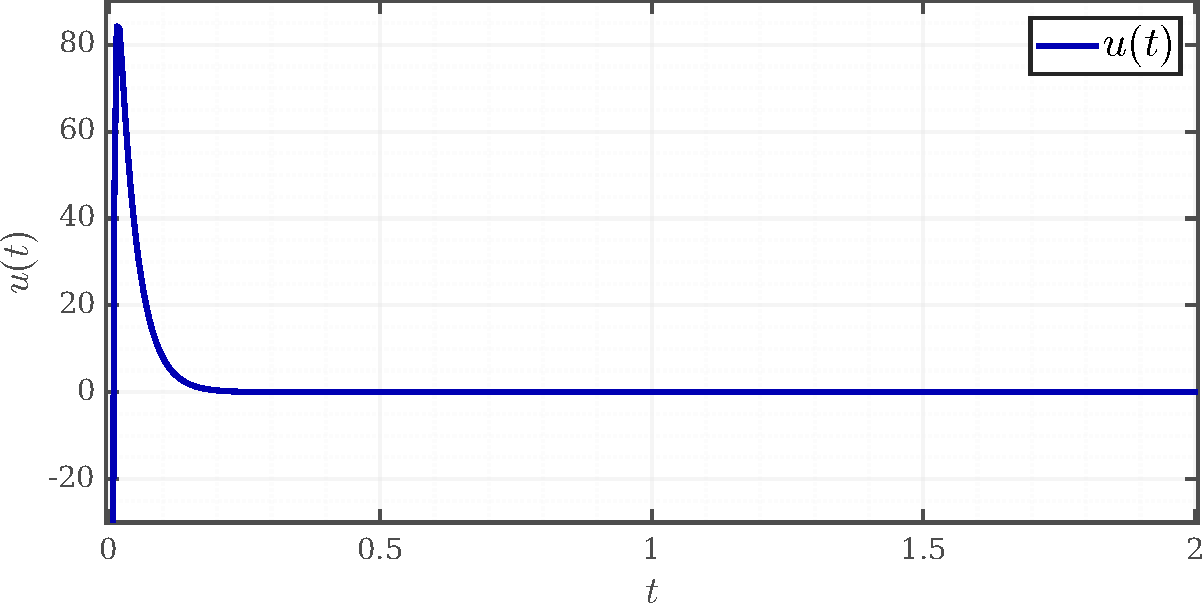
\includegraphics[width=0.9\textwidth]{../images/task1/u2.pdf}
	\caption{Управление \(u(t)\)}
	\label{fig:u12}
\end{figure}

Все компоненты вектора состояния асимптотически сходятся 
к нулю, что подтверждает корректность синтеза. Управление 
$u(t)$ также стремится к нулю.


\subsection{Метод Басса-Гура\(\mathbb{/}\)Аккермана (спектр $\{-3,\ -3 \pm 9i\}$)}
Аналогично предыдущим методам возьму от систему управляемую усеченную часть, синтезирую матрицу \(\hat K_c\), дополню ее недостающим нулем, соответствующим неуправляемому собственному числу матрицы системы и перейду в исходный базис из жорданового и получу искомую матрицу \(K\).\\
Синтезирую матрицу $\hat{K}_c$ по формуле Басса-Гура:
\[
\hat{K}_c = -\bar{a} A_a^{-1} \hat{U}_c^{-1}
\]
Запишу характеристический полином матрицы с желаемым спектром (матрица будет усеченной). Найду коэффициенты полинома:
\[
D^*(\lambda) = (\lambda + 3 - 9i)(\lambda + 3 + 9i) = \lambda^2 + 6\lambda + 90
\]
Также найду коэффициенты полинома \(D(\lambda)\) -- это полином усеченной матрицы системы:
\[
D(\lambda) = \lambda^2 -4 \lambda + 8
\]
Запишу матрицу \(\bar a\) - матрица разности коэффициентов полиномов \(D^*(\lambda)\) и \(D(\lambda)\):
\[
\bar a = \begin{bmatrix}
	6 - (-4) & 90 - 8 \\
\end{bmatrix} = \begin{bmatrix}
	10 & 82 \\
\end{bmatrix}
\]
Составлю матрицу $A_a$ из коэффициентов полинома $D(\lambda)$:
\[
A_a = \begin{bmatrix}
	1 & -4 \\
	0 & 1
\end{bmatrix}
\]
Найду матрицу управляемости $\hat{U}_c$ (листинг~\ref{lst:P1}):
\[
\hat{U}_c = \begin{bmatrix}
	\hat{B}_c & \hat{A}_c \hat{B}_c
\end{bmatrix} = \begin{bmatrix}
	2.12 & -5.66 \\
	4.95 & 14.14
\end{bmatrix}
\]
Посчитаю значение \(\hat K_c\) програмно (листинг~\ref{lst:bassa}):
\[
\hat K_c = \begin{bmatrix}
	7.97 & -5.44 \\
\end{bmatrix}
\]
Переведу матрицу в исходный и расширенный базис (листинг~\ref{lst:origK11}, аналогично):
\[
\hat K =
\begin{bmatrix}
	0 & 7.97 & -5.44
\end{bmatrix}
\qquad \Longrightarrow \qquad	
K = \begin{bmatrix} -7.69 & -1.79 & -7.69 \end{bmatrix}
\]
Проверю корректность расчетов. Найду матрицу замкнутой системы и ее собственные числа, сравню с желаемыми (листинг~\ref{lst:eig1}, аналогично):
\[
A + BK = \begin{bmatrix}
	
	15.69 & 2.79 & 18.69 \\
	27.07 & 5.38 & 27.07 \\
	-27.07 & -8.38 & -30.07 \\
\end{bmatrix} \qquad 
\sigma(A + BK) = \{-3,\ -3 \pm 9i\}
\]

Желаемый и полученный спектры совпадают, матрица \(K\) найдена верно. 	


Выполню компьютерное моделирование замкнутой системы при начальных условиях 
$x(0) = \begin{bmatrix} 1 & 1 & 1 \end{bmatrix}^\top$. 
Результаты представлены на рисунках~\ref{fig:x13} и~\ref{fig:u13}:

\begin{figure}[H]
	\centering
	
\includegraphics[width=0.9\textwidth]{../images/task1/x3.pdf}
	\caption{Вектор состояния \(x(t)\)}
	\label{fig:x13}
\end{figure}

\begin{figure}[H]
	\centering
	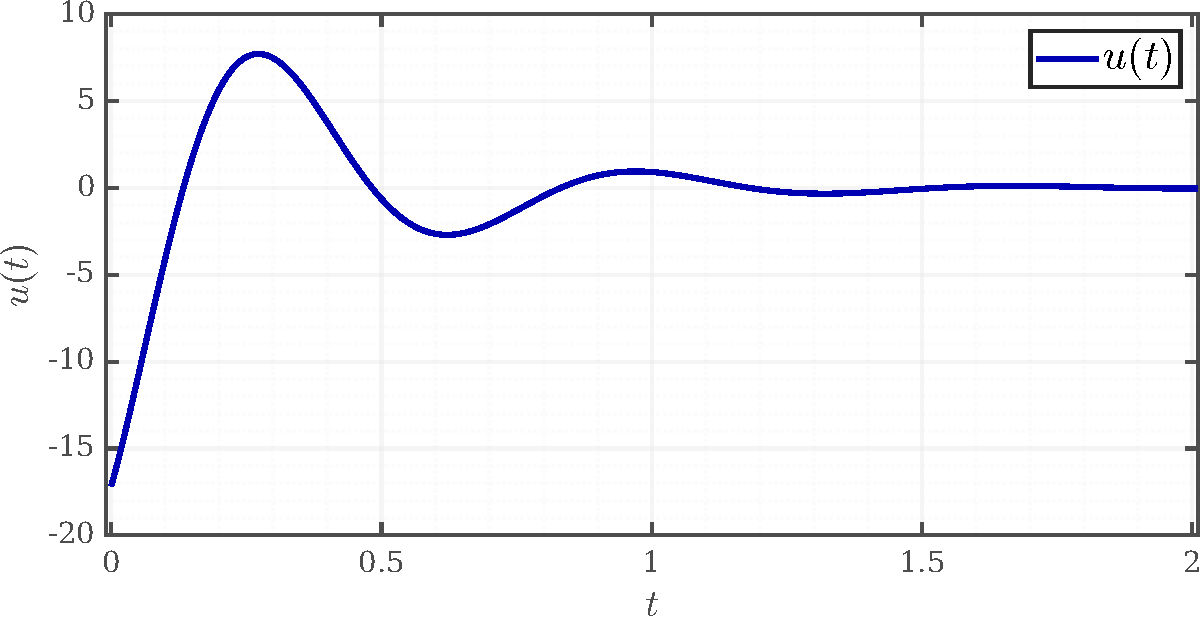
\includegraphics[width=0.9\textwidth]{../images/task1/u3.pdf}
	\caption{Управление \(u(t)\)}
	\label{fig:u13}
\end{figure}

Все компоненты вектора состояния асимптотически сходятся 
к нулю, что подтверждает корректность синтеза. Управление 
$u(t)$ также стремится к нулю.


\newpage
\subsection{Вывод по заданию}

В задании я синтезировала модальные регуляторы для системы. Поскольку система была не полностью управляемой, все методы применялись к усечённой управляемой части после перехода к вещественной жордановой форме, что упростило расчёты за счёт уменьшения размерности.

Метод Сильвестра оказался наиболее теоретически сложным, метод модального управления потребовал наибольшего числа преобразований, а метод Басса--Гура\(/\)Аккермана оказался самым простым в реализации благодаря прямой аналитической формуле.\\

По результатам моделирования видно, что при увеличении модулей желаемых собственных чисел возрастают коэффициенты матрицы обратной связи $K$ и амплитуда управляющего воздействия, поскольку для более быстрого перемещения собственных чисел требуется более сильное управление. Сравнение всех сигналов управления приведено на рисунке~\ref{fig:u1123}.

\begin{figure}[H]
	\centering
	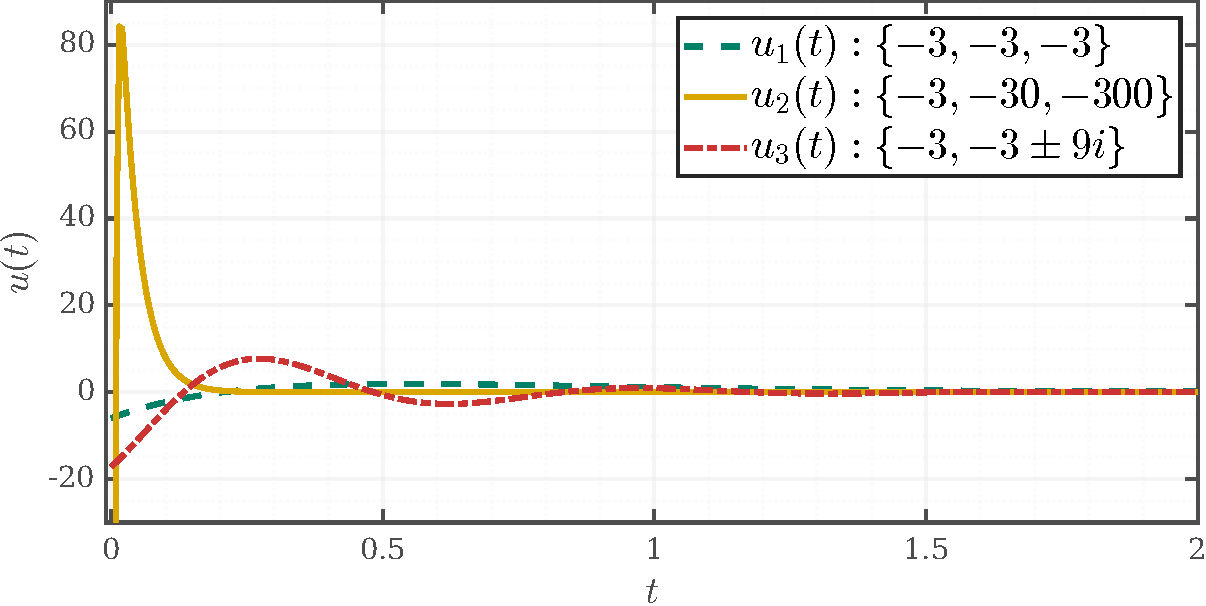
\includegraphics[width=0.9\textwidth]{../images/task1/u123.pdf}
	\caption{Управление \(u_1(t), u_2(t), u_3(t)\)}
	\label{fig:u1123}
\end{figure}

\newpage
\section{Наблюдатель полного порядка}
\label{sec:task2}

В соответствии с вариантом рассмотрю систему:

\[
\begin{cases}
	\dot{x} = Ax \\
	y = Cx
\end{cases}
\]

где

\[
A =
\begin{bmatrix}
	-40 & 16  &  9  &  7 \\
	-64 & 25  & 14  & 12 \\
	-26 & 11  &  7  &  3 \\
	-48 & 18  & 14  &  8
\end{bmatrix}
\qquad
C^{\top} =
\begin{bmatrix}
	-3 \\ 2 \\ -2 \\ 1
\end{bmatrix}
\]

Требуется:

\begin{itemize}
	\item Найти собственные числа матрицы $A$, определить наблюдаемость и обнаруживаемость системы.
	\item Построить схему моделирования системы с наблюдателем состояния
	$\dot{\hat{x}} = A\hat{x} + L(C\hat{x} - y)$.
	\item Для каждого из спектров:
	\begin{itemize}
		\item Синтезировать матрицу коррекции наблюдателя $L$.
		\item Определить собственные числа матрицы $(A + LC)$ и сравнить с желаемым спектром.
		\item Выполнить моделирование при
		$x(0) = \begin{bmatrix}1&1&1&1\end{bmatrix}^{\top}$,
		$\hat{x}(0) = \begin{bmatrix}0&0&0&0\end{bmatrix}^{\top}$,
		построить сравнительные графики $x(t)$ и $\hat{x}(t)$,
		а также график ошибки $e(t) = x(t) - \hat{x}(t)$.
	\end{itemize}
	\item Сопоставить результаты для различных спектров, выявить преимущества и недостатки каждого.
\end{itemize}

\hrule \newpage

\subsection{Анализ системы}

Найду собственные числа матрицы \(A\) (листинг~\ref{lst:eig2}):

\[
A =
\begin{bmatrix}
	-40 & 16  &  9  &  7 \\
	-64 & 25  & 14  & 12 \\
	-26 & 11  &  7  &  3 \\
	-48 & 18  & 14  &  8
\end{bmatrix} 
\qquad \Longrightarrow \qquad
\sigma(A) = \{\pm 2i, \pm 3i\}
\]

Чтобы оценить наблюдаемость каждого собственного числа переведу систему в Жорданову форму (листинг~\ref{lst:jordan2}). Получаю:

\[
\begin{cases}
	\dot{\tilde{x}} =
	\begin{bNiceMatrix}[create-medium-nodes, left-margin=4pt, right-margin=4pt]
		0 & -2 &  0 &  0 \\
		2 &  0 &  0 &  0 \\
		0 &  0 &  0 & -3 \\
		0 &  0 &  3 &  0 \\
		\CodeAfter
		\tikz \draw[green!40!black, rounded corners=4pt, line width=0.7pt, opacity=0.4]
		([xshift=-2pt, yshift=2pt]1-1-medium.north west) rectangle
		([xshift=2pt, yshift=-2pt]2-2-medium.south east);
		\tikz \draw[green!40!black, rounded corners=4pt, line width=0.7pt, opacity=0.4]
		([xshift=-2pt, yshift=2pt]3-3-medium.north west) rectangle
		([xshift=2pt, yshift=-2pt]4-4-medium.south east);
	\end{bNiceMatrix}
	\tilde{x} \\[30pt]
	y =
	\begin{bNiceMatrix}[create-medium-nodes, left-margin=4pt, right-margin=4pt]
		14.14 & -7.07 & -11.31 & 2.12 \\
		\CodeAfter
		\tikz \draw[green!40!black, rounded corners=4pt, line width=0.7pt, opacity=0.4]
		([xshift=-2pt, yshift=2pt]1-1-medium.north west) rectangle
		([xshift=2pt, yshift=-2pt]1-2-medium.south east);
		\tikz \draw[green!40!black, rounded corners=4pt, line width=0.7pt, opacity=0.4]
		([xshift=-2pt, yshift=2pt]1-3-medium.north west) rectangle
		([xshift=2pt, yshift=-2pt]1-4-medium.south east);
	\end{bNiceMatrix}
	\hat{x}
\end{cases}
\]

Так как первые элементы матрицы \(\hat C\), соответствующие жордановым блокам ненулевые, система полностью наблюдаема. А значит, все собственные числа также наблюдаемы.

Поскольку система полностью наблюдаема, то она обнаруживаема.

\subsection{Схема моделирования системы}

Построю схему замкнутой системы:

\[
\begin{cases}
	\dot{x} = Ax, \\
	\dot{\hat{x}} = (A + LC)\hat{x} - LCx.
\end{cases}
\]

\begin{figure}[H]
	\centering
	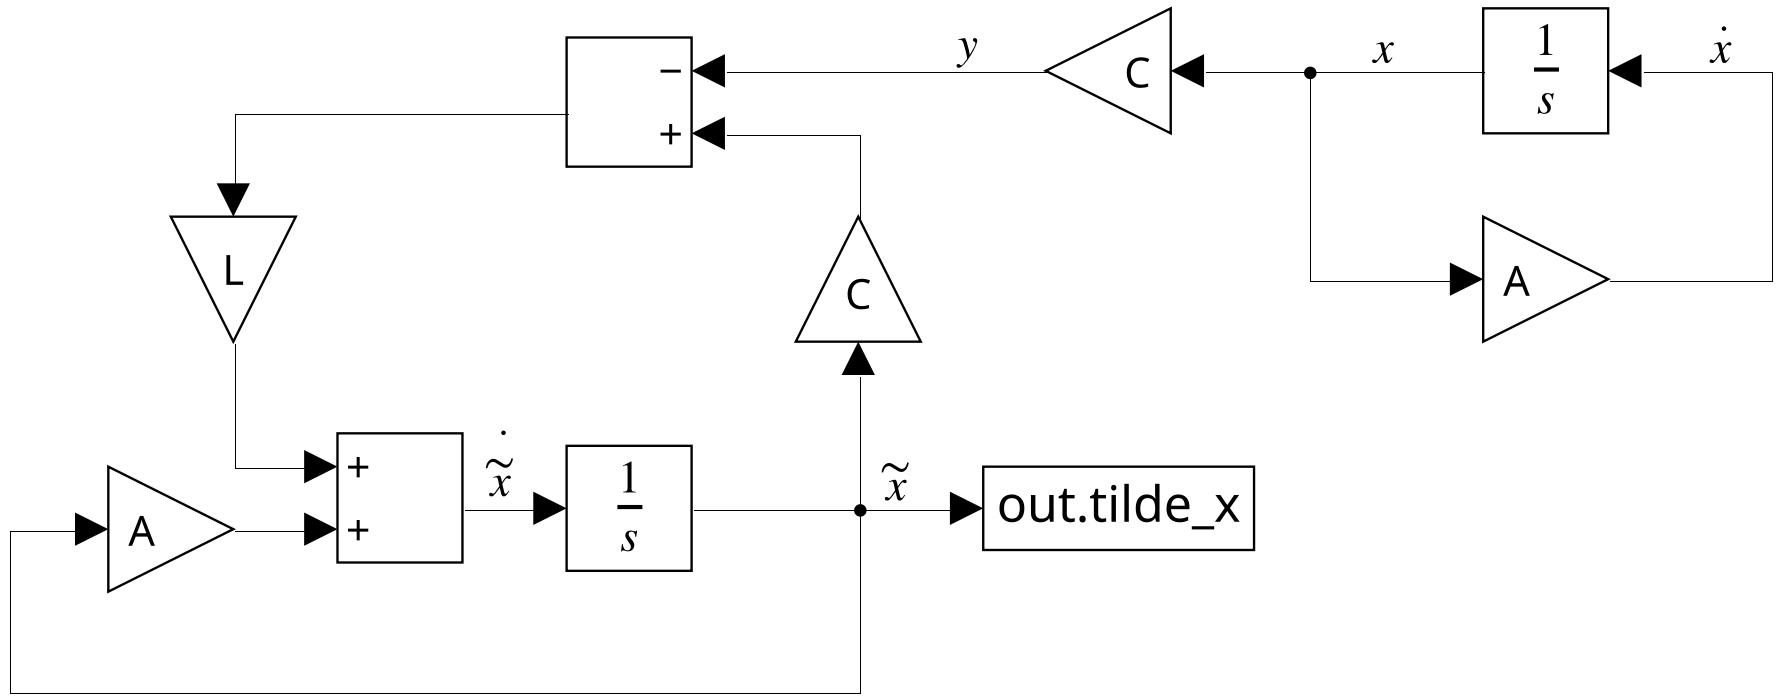
\includegraphics[width=0.9\textwidth]{../images/task2/model2.png}
	\caption{Структурная схема замкнутой системы}
\end{figure}


\subsection{Анализ спектра \(\{-1, -1, -1, -1\}\)}

Для начала запишу желаемый характеристический полином наблюдателя:

\[
D(\lambda) = (\lambda + 1)^4 = \lambda^4 + 4\lambda^3 + 6\lambda^2 + 4\lambda + 1
\]

Запишу матрицу \(\Gamma\) в канонической наблюдаемой форме:

\[
\Gamma = 
\begin{bmatrix}
	0 & 0 & 0 & -1 \\
	1 & 0 & 0 & -4 \\
	0 & 1 & 0 & -6 \\
	0 & 0 & 1 & -4
\end{bmatrix}
\]

Теперь переведу систему в каноническую наблюдаемую форму (листинг~\ref{lst:kanon2}). Получаю:

\[
\begin{cases}
	\dot{x_k} = \begin{bmatrix}
		0 & 0 & 0  & -36 \\
		1 & 0 & 0 & 0 \\
		0 & 1 & 0 & -13 \\
		0 & 0 & 1 & 0 \\
	\end{bmatrix} x_k \\[30pt]
	y = \begin{bmatrix}
		1 & 0 & 0 & 0
	\end{bmatrix} x_k
\end{cases}
\]

Найду матрицу $L_k$ в канонической наблюдаемой форме из условия:
\[
A_k + L_k C_k = \Gamma
\]

Поскольку это громоздко вручную, поэтому решу в MATLAB (листинг~\ref{lst:lk}):

\[L_k =   \begin{bmatrix}
	35 \\ -4 \\ 7 \\ -4 
\end{bmatrix}\]

Для перехода из канонического базиса в исходный использую матрицу перехода
через матрицы наблюдаемости (листинг~\ref{lst:lobs}):
\[
T = V(A_k,\, C_k)^{-1} V(A,\, C) \qquad L = T^{-1} L_k
\]

Получаю матрицу \(L\):

\[L =   \begin{bmatrix}
	33.23 \\ -53.4 \\ -22.57 \\ -42.03
\end{bmatrix}\]

Проверю достигнут ли желаемый спектр при найденной матрице L (листинг~\ref{lst:check}). Матрица замкнутой системы:

\[
A + L C = \begin{bmatrix}
	59.70 & -50.47 & 75.47 & -26.23 \\
	96.20 & -81.80 & 120.80 & -41.40 \\
	41.70 & -34.13 & 52.13 & -19.57 \\
	78.10 & -66.07 & 98.07 & -34.03
\end{bmatrix}
\]

Спектр матрицы замкнутой системы:

\[
\sigma(A + L C) = \{-1, -1, -1, -0.99\}
\]

Небольшое отклонение от желаемого спектра можно объяснить численной погрешностью при вычислении кратных собственных чисел. \\

Выполню компьютерное моделирование при начальных условиях
$x(0) = \begin{bmatrix} 1 & 1 & 1 & 1 \end{bmatrix}^\top$,
$\hat{x}(0) = \begin{bmatrix} 0 & 0 & 0 & 0 \end{bmatrix}^\top$
и построю сравнительные графики $x(t)$ и $\hat{x}(t)$,
а также график ошибки наблюдателя $e(t) = x(t) - \hat{x}(t)$
(рисунки~\ref{fig:x_xhat_1} и~\ref{fig:e_1}).

Также построю приближенный график векторов состояния, чтобы показать, что начальные условия системы и наблюдателя различаются. Начальные условия покажу пунктирными линиями соответствующего цвета.

\begin{figure}[H]
	\centering
	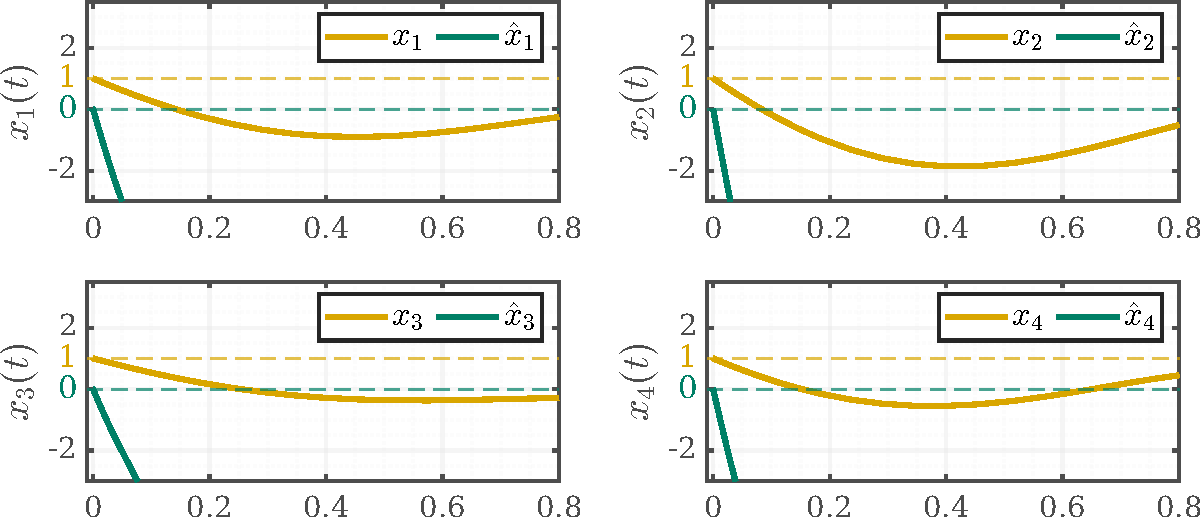
\includegraphics[width=0.9\textwidth]{../images/task2/xp1.pdf}
	\caption{Приближенный вектор состояния $x(t)$ и $\hat{x}(t)$}
	\label{fig:x_xhat_p_1}
\end{figure}

\begin{figure}[H]
	\centering
	\begin{subfigure}[b]{0.45\textwidth}
		\centering
		
\includegraphics[width=\textwidth]{../images/task2/x1.pdf}
		\caption{Вектор состояния $x(t)$ и $\hat{x}(t)$}
		\label{fig:x_xhat_1}
	\end{subfigure}
	\hfill
	\begin{subfigure}[b]{0.45\textwidth}
		\centering
		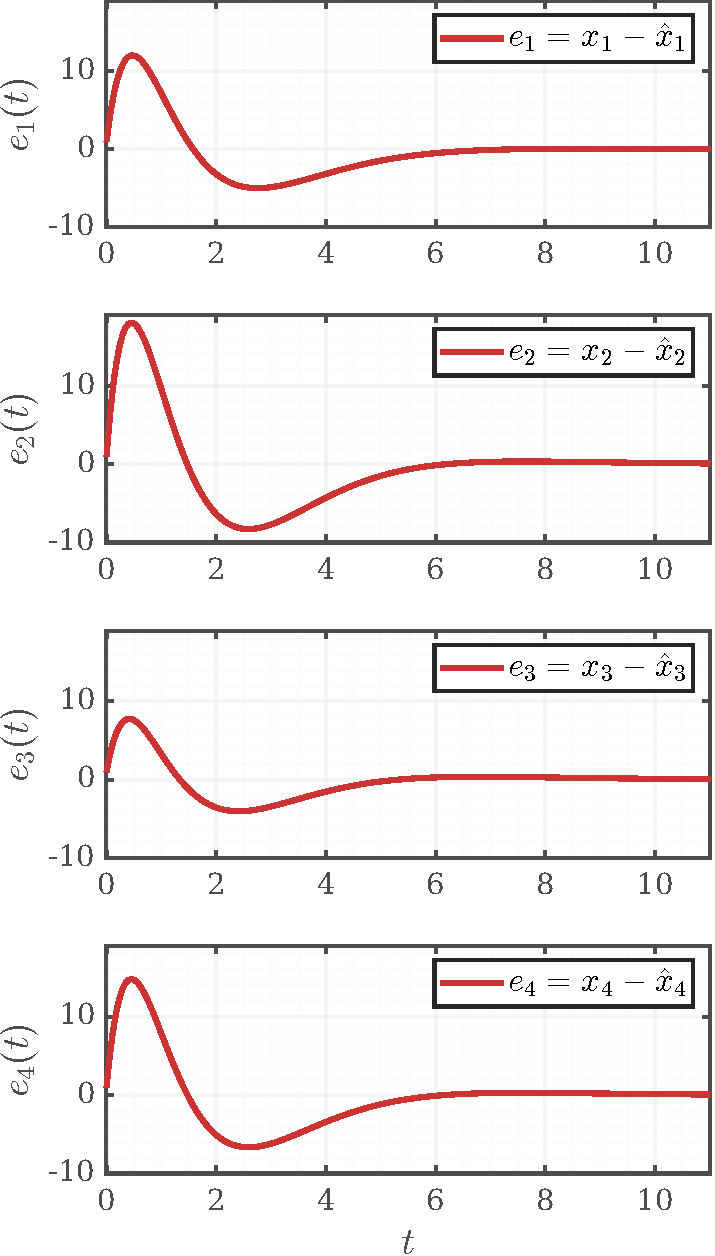
\includegraphics[width=\textwidth]{../images/task2/e1.pdf}
		\caption{Ошибка наблюдения $e(t)$}
		\label{fig:e_1}
	\end{subfigure}
	\caption{Спектр $\{-1, -1, -1, -1\}$}
	\label{fig:obs_spec1}
\end{figure}



Система имеет чисто мнимые собственные числа $\sigma(A) = \{\pm 2i, \pm 3i\}$, поэтому вектор состояния $x(t)$ не затухает и не расходится, а колеблется. Наблюдатель с выбранным спектром успешно справляется со своей задачей — ошибка $e(t)$ асимптотически стремится к нулю, то есть $\hat{x}(t)$ догоняет $x(t)$ и точно воспроизводит его колебания.

\subsection{Анализ спектра \(\{-1, -10, -100, -100\}\)}

Запишу характеристическое уравнение матрицы с желаемым спектром:

\[
D(\lambda) = (\lambda + 1)(\lambda + 10)(\lambda + 100)^2
= \lambda^4 + 211\lambda^3 + 11110\lambda^2 + 111000\lambda + 100000
\]

Матрица \(\Gamma\) с желаемым спектром в канонической наблюдаемой форме:

\[
\Gamma = 
\begin{bmatrix}
	0 & 0 & 0 & -100000 \\
	1 & 0 & 0 & -111000 \\
	0 & 1 & 0 & -11110  \\
	0 & 0 & 1 & -211
\end{bmatrix}
\]


Матрицы системы в канонической наблюдаемой форме уже были найдены, поэтому приступлю у поиску$L_k$ в канонической наблюдаемой форме (листинг~\ref{lst:lk}, аналогично):

\[
A_k + L_k C_k = \Gamma
\qquad \Longrightarrow \qquad
L_k =   \begin{bmatrix}
	-99964 \\ -112000 \\ 12197 \\ -211 
\end{bmatrix}
\]

Через матрицу перехода \(T\), составленную при помощи матриц наблюдаемости найду \(L\) в исходном базисе (листинг~\ref{lst:lobs}, аналогично):

\[
L = 10^5 \cdot \begin{bmatrix}
	1.61 \\
	2.56 \\
	1.17 \\
	2.06
\end{bmatrix}
\]

Проверю достигнут ли желаемый спектр при найденной матрице L (листинг~\ref{lst:check}, аналогично). Матрица замкнутой системы:

\[
A + LC = 10^5 \cdot
\begin{bmatrix}
	-4.84 &  3.23 & -3.23 &  1.61 \\
	-7.67 &  5.11 & -5.11 &  2.56 \\
	-3.50 &  2.33 & -2.33 &  1.17 \\
	-6.17 &  4.11 & -4.11 &  2.06
\end{bmatrix}
\]

Спектр матрицы замкнутой системы:

\[
\sigma(A + L C) = \{-100.01, -99.99, -10, -1\}
\]

Небольшое отклонение от желаемого спектра можно объяснить численной погрешностью при вычислении кратных собственных чисел. \\


Выполню компьютерное моделирование при начальных условиях
$x(0) = \begin{bmatrix} 1 & 1 & 1 & 1 \end{bmatrix}^\top$,
$\hat{x}(0) = \begin{bmatrix} 0 & 0 & 0 & 0 \end{bmatrix}^\top$
и построю сравнительные графики $x(t)$ и $\hat{x}(t)$,
а также график ошибки наблюдателя $e(t) = x(t) - \hat{x}(t)$
(рисунки~\ref{fig:x_xhat_2} и~\ref{fig:e_2}).

Также построю приближенный график векторов состояния, чтобы показать, что начальные условия системы и наблюдателя различаются. Начальные условия покажу пунктирными линиями соответствующего цвета.

\begin{figure}[H]
	\centering
	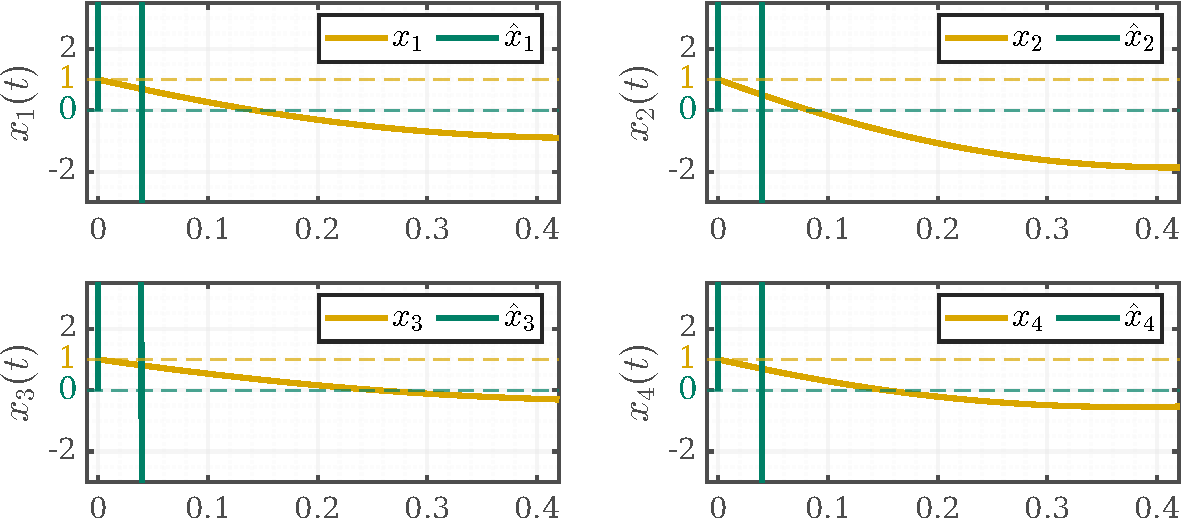
\includegraphics[width=0.95\textwidth]{../images/task2/xp2.pdf}
	\caption{Приближенный вектор состояния $x(t)$ и $\hat{x}(t)$}
	\label{fig:x_xhat_p_2}
\end{figure}

\begin{figure}[H]
	\centering
	\begin{subfigure}[b]{0.49\textwidth}
		\centering
		
\includegraphics[width=\textwidth]{../images/task2/x2.pdf}
		\caption{Вектор состояния $x(t)$ и $\hat{x}(t)$}
		\label{fig:x_xhat_2}
	\end{subfigure}
	\hfill
	\begin{subfigure}[b]{0.49\textwidth}
		\centering
		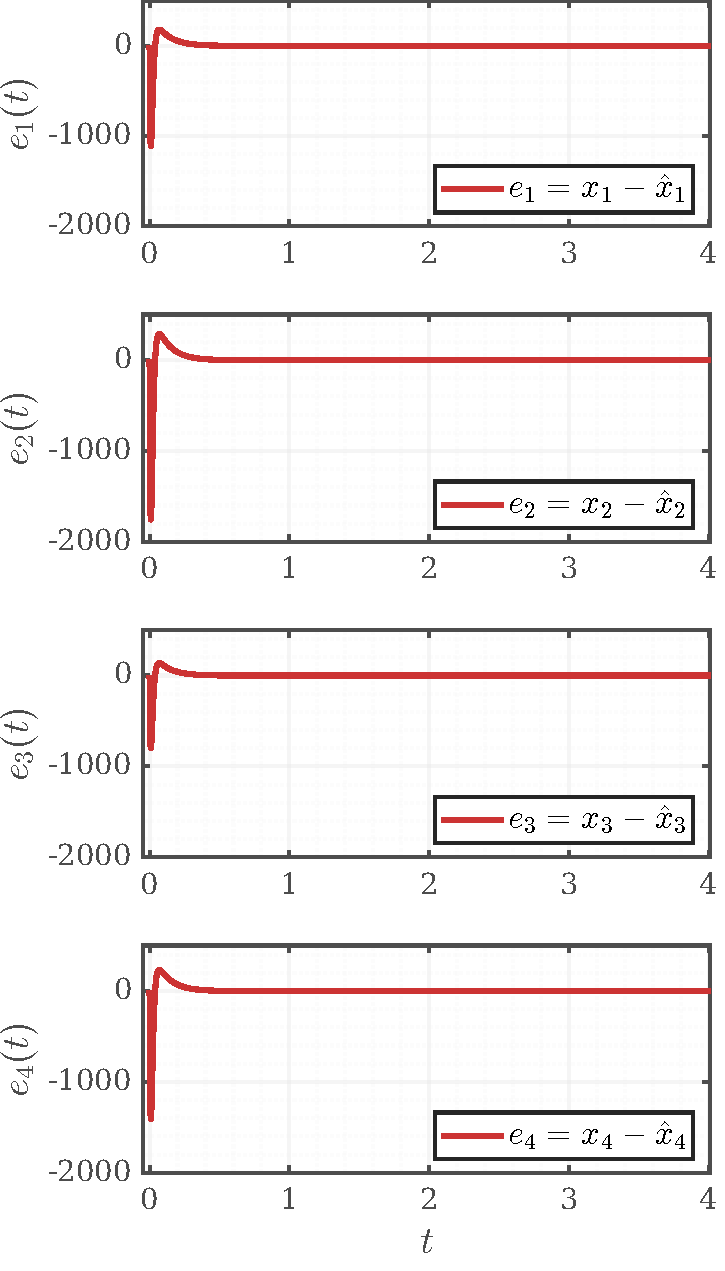
\includegraphics[width=\textwidth]{../images/task2/e2.pdf}
		\caption{Ошибка наблюдения $e(t)$}
		\label{fig:e_2}
	\end{subfigure}
	\caption{Спектр $\{-1, -10, -100, -100\}$}
	\label{fig:obs_spec2}
\end{figure}


Наблюдатель с выбранным спектром успешно справляется 
со своей задачей --- ошибка $e(t)$ асимптотически стремится к нулю значительно 
быстрее, чем в случае спектра $\{-1,-1,-1,-1\}$, однако за счёт более удалённых 
от мнимой оси собственных чисел матрица коррекции $L$ содержит существенно 
большие коэффициенты.

\subsection{Анализ спектра \(\{-1 \pm 2i, -1 \pm 3i\}\)}

Запишу желаемый характеристический полином наблюдателя:
\[
\begin{aligned}
	D(\lambda) &= (\lambda + 1 - 2i)(\lambda + 1 + 2i)(\lambda + 1 - 3i)(\lambda + 1 + 3i) \\
	&= (\lambda^2 + 2\lambda + 5)(\lambda^2 + 2\lambda + 10) \\
	&= \lambda^4 + 4\lambda^3 + 19\lambda^2 + 30\lambda + 50
\end{aligned}
\]

Матрица $\Gamma$ с желаемым спектром в канонической наблюдаемой форме:
\[
\Gamma = 
\begin{bmatrix}
	0 & 0 & 0 & -50 \\
	1 & 0 & 0 & -30 \\
	0 & 1 & 0 & -19 \\
	0 & 0 & 1 & -4
\end{bmatrix}
\]

Матрицы системы в канонической наблюдаемой форме уже были найдены, поэтому
приступлю к поиску $L_k$ в канонической наблюдаемой форме (листинг~\ref{lst:lk}, аналогично):
\[
A_k + L_k C_k = \Gamma
\qquad \Longrightarrow \qquad
L_k = \begin{bmatrix}
	-14 \\ -30 \\ -6 \\ -4
\end{bmatrix}
\]
Через матрицу перехода $T$, составленную при помощи матриц наблюдаемости,
найду $L$ в исходном базисе (листинг~\ref{lst:lobs}, аналогично):
\[
L = \begin{bmatrix}
	11.93 \\ 16.80 \\ 7.67 \\ 13.53
\end{bmatrix}
\]
Проверю достигнут ли желаемый спектр при найденной матрице $L$
(листинг~\ref{lst:check}, аналогично):
\[ A + LC =
\begin{bmatrix}
	-24.07 &  16.00 & -14.87 &  10.93 \\
	-17.60 &  25.00 & -17.60 &  12.80 \\
	-12.00 &  11.00 &  -7.33 &   8.47 \\
	-26.60 &  18.00 & -12.53 &  21.53
\end{bmatrix}
\qquad \Longrightarrow \qquad
\sigma(A + LC) = \{-1 \pm 2i,\ -1 \pm 3i\}
\]
Желаемый спектр достигнут точно.\\

Выполню компьютерное моделирование при начальных условиях
$x(0) = \begin{bmatrix} 1 & 1 & 1 & 1 \end{bmatrix}^\top$,
$\hat{x}(0) = \begin{bmatrix} 0 & 0 & 0 & 0 \end{bmatrix}^\top$
и построю сравнительные графики $x(t)$ и $\hat{x}(t)$,
а также график ошибки наблюдателя $e(t) = x(t) - \hat{x}(t)$
(рисунки~\ref{fig:x_xhat_3} и~\ref{fig:e_3}).

Также построю приближенный график векторов состояния, чтобы показать, что начальные условия системы и наблюдателя различаются. Начальные условия покажу пунктирными линиями соответствующего цвета.

\begin{figure}[H]
	\centering
	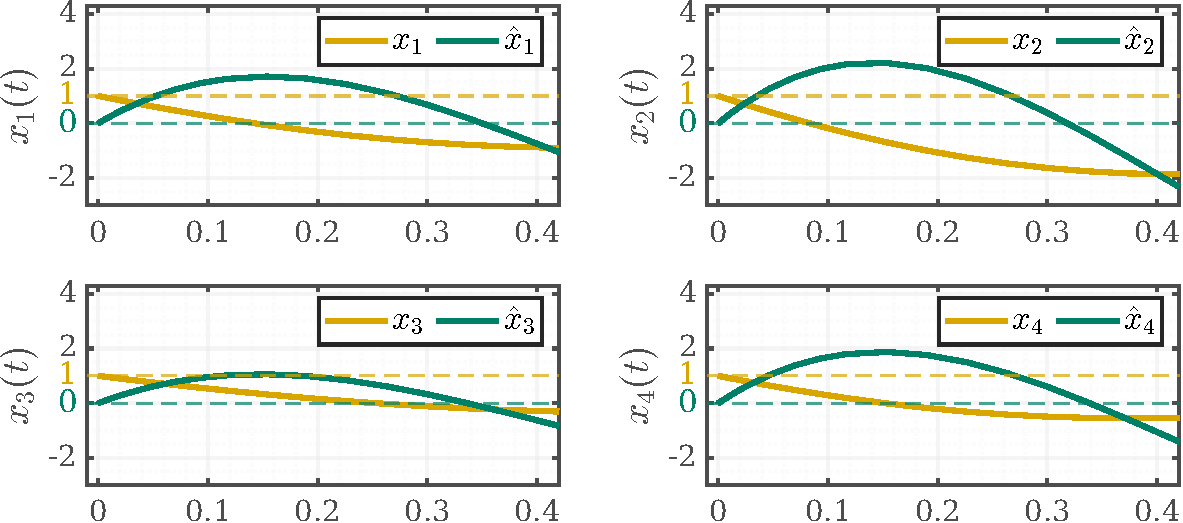
\includegraphics[width=0.9\textwidth]{../images/task2/xp3.pdf}
	\caption{Приближенный вектор состояния $x(t)$ и $\hat{x}(t)$}
	\label{fig:x_xhat_p_3}
\end{figure}

\begin{figure}[H]
	\centering
	\begin{subfigure}[b]{0.43\textwidth}
		\centering
		
\includegraphics[width=\textwidth]{../images/task2/x3.pdf}
		\caption{Вектор состояния $x(t)$ и $\hat{x}(t)$}
		\label{fig:x_xhat_3}
	\end{subfigure}
	\hfill
	\begin{subfigure}[b]{0.43\textwidth}
		\centering
		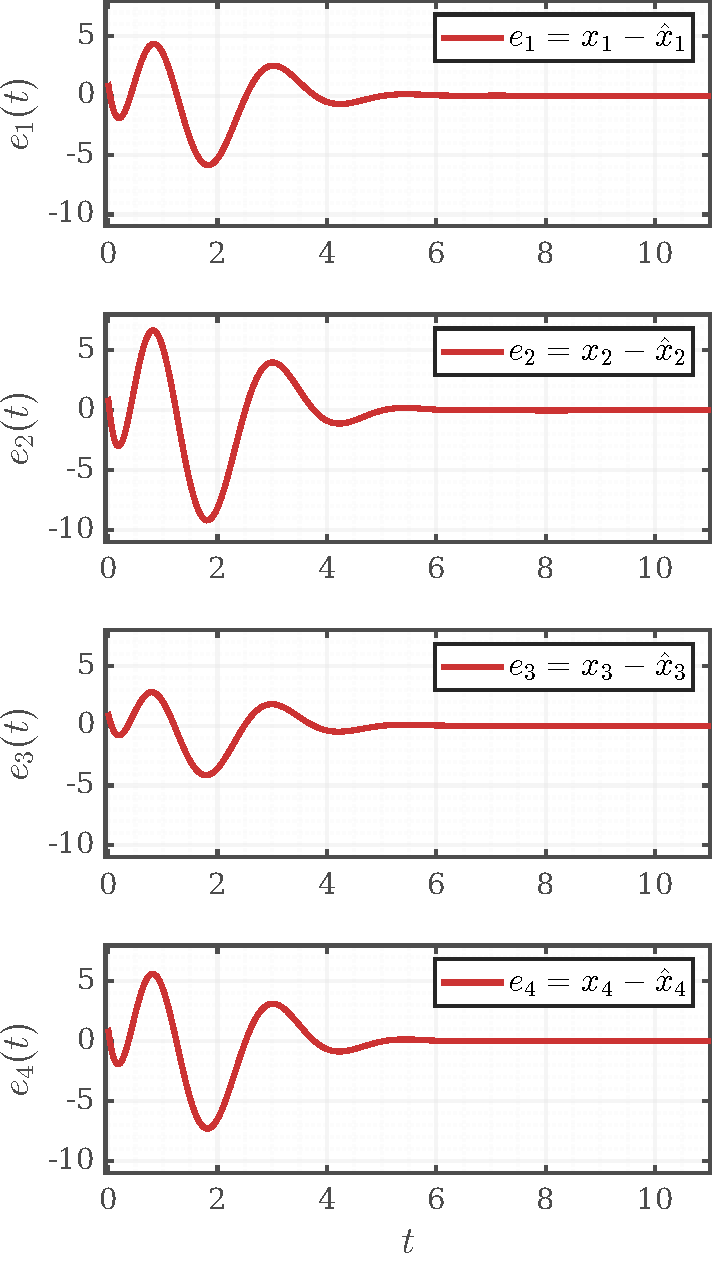
\includegraphics[width=\textwidth]{../images/task2/e3.pdf}
		\caption{Ошибка наблюдения $e(t)$}
		\label{fig:e_3}
	\end{subfigure}
	\caption{Спектр $\{-1 \pm 2i, -1 \pm 3i\}$}
	\label{fig:obs_spec3}
\end{figure}


Наблюдатель с выбранным спектром $\{-1\pm 2i,\ -1\pm 3i\}$ успешно справляется 
со своей задачей --- ошибка $e(t)$ асимптотически стремится к нулю. При этом коэффициенты матрицы $L$ значительно 
меньше, чем для спектра $\{-1,-10,-100,-100\}$.

\newpage
\subsection{Вывод по заданию}

Все три наблюдателя успешно справились с задачей: ошибка $e(t)$
асимптотически стремится к нулю. Спектр $\{-1,-1,-1,-1\}$ обеспечивает
медленную сходимость при малых коэффициентах $L$; спектр
$\{-1,-10,-100,-100\}$ даёт быструю сходимость; у спектра $\{-1\pm 2i,\ -1\pm 3i\}$ ошибка также асимптотически сходится к нулю.


\newpage
\section{Модальное управление по выходу}
\label{sec:task3}

В соответствии с вариантом рассмотрю систему:

\[
\begin{cases}
	\dot{x} = Ax + Bu \\
	y = Cx + Du
\end{cases}
\]

где

\[
A =
\begin{bmatrix}
	5 & -9 & -7 &  1 \\
	-9 &  5 & -1 &  7 \\
	-7 & -1 &  5 &  9 \\
	1 &  7 &  9 &  5
\end{bmatrix}
\qquad
B =
\begin{bmatrix}
	3 \\ 3 \\ 1 \\ 3
\end{bmatrix}
\qquad
C =
\begin{bmatrix}
	2 & -2 & 2 & 2 \\
	-2 &  4 & 2 & 4
\end{bmatrix}
\qquad
D =
\begin{bmatrix}
	4 \\ 1
\end{bmatrix}
\]

Требуется:

\begin{itemize}
	\item Найти собственные числа матрицы $A$, определить управляемость и наблюдаемость каждого из них, сделать вывод о стабилизируемости и обнаруживаемости системы.
	\item Построить схему моделирования системы, замкнутой наблюдателем $\dot{\hat{x}} = A\hat{x} + (B + LD)u + L(C\hat{x} - y)$ и законом управления $u = K\hat{x}$.
	\item Задаться достижимыми желаемыми спектрами регулятора и наблюдателя.
	\item Синтезировать $K$ и $L$, проверить спектры $(A + BK)$ и $(A + LC)$.
	\item Выполнить моделирование при $x(0) = \begin{bmatrix}1&1&1&1\end{bmatrix}^{\top}$, $\hat{x}(0) = \begin{bmatrix}0&0&0&0\end{bmatrix}^{\top}$, построить графики $u(t)$, $y(t)$, $x(t)$, $\hat{x}(t)$ и $e(t) = x(t) - \hat{x}(t)$.
\end{itemize}

\hrule \newpage

\subsection{Анализ системы}

Найду собственные числа матрицы $A$ (листинг~\ref{lst:eig3}):

\[
A =
\begin{bmatrix}
	5 & -9 & -7 &  1 \\
	-9 &  5 & -1 &  7 \\
	-7 & -1 &  5 &  9 \\
	1 &  7 &  9 &  5
\end{bmatrix}
\qquad \Longrightarrow \qquad
\sigma(A) = \{-12,\ 4,\ 8,\ 20\}
\]

Все собственные числа вещественные и различные, следовательно, жорданова форма диагональна.
Чтобы оценить управляемость и наблюдаемость каждого из них, переведу систему в жорданов базис (листинг~\ref{lst:jordan3}):

\[
\begin{cases}
	\dot{\tilde{x}} =
	\begin{bNiceMatrix}[create-medium-nodes, left-margin=4pt, right-margin=4pt]
		-12 &  0 &  0 &  0 \\
		0 &  4 &  0 &  0 \\
		0 &  0 &  8 &  0 \\
		0 &  0 &  0 & 20 \\
		\CodeAfter
		\tikz \draw[green!40!black, rounded corners=3pt, line width=0.7pt, opacity=0.4]
		([xshift=-2pt, yshift=2pt]1-1-medium.north west) rectangle
		([xshift=2pt, yshift=-2pt]1-1-medium.south east);
		\tikz \draw[green!40!black, rounded corners=3pt, line width=0.7pt, opacity=0.4]
		([xshift=-2pt, yshift=2pt]2-2-medium.north west) rectangle
		([xshift=2pt, yshift=-2pt]2-2-medium.south east);
		\tikz \draw[green!40!black, rounded corners=3pt, line width=0.7pt, opacity=0.4]
		([xshift=-2pt, yshift=2pt]3-3-medium.north west) rectangle
		([xshift=2pt, yshift=-2pt]3-3-medium.south east);
		\tikz \draw[green!40!black, rounded corners=3pt, line width=0.7pt, opacity=0.4]
		([xshift=-2pt, yshift=2pt]4-4-medium.north west) rectangle
		([xshift=2pt, yshift=-2pt]4-4-medium.south east);
	\end{bNiceMatrix}
	\tilde{x}
	+
	\begin{bNiceMatrix}[create-medium-nodes, left-margin=4pt, right-margin=4pt]
		-2 \\ -4 \\ 2 \\ 2 \\
		\CodeAfter
		\tikz \draw[green!40!black, rounded corners=3pt, line width=0.7pt, opacity=0.4]
		([xshift=-2pt, yshift=2pt]1-1-medium.north west) rectangle
		([xshift=2pt, yshift=-2pt]1-1-medium.south east);
		\tikz \draw[green!40!black, rounded corners=3pt, line width=0.7pt, opacity=0.4]
		([xshift=-2pt, yshift=2pt]2-1-medium.north west) rectangle
		([xshift=2pt, yshift=-2pt]2-1-medium.south east);
		\tikz \draw[green!40!black, rounded corners=3pt, line width=0.7pt, opacity=0.4]
		([xshift=-2pt, yshift=2pt]3-1-medium.north west) rectangle
		([xshift=2pt, yshift=-2pt]3-1-medium.south east);
		\tikz \draw[green!40!black, rounded corners=3pt, line width=0.7pt, opacity=0.4]
		([xshift=-2pt, yshift=2pt]4-1-medium.north west) rectangle
		([xshift=2pt, yshift=-2pt]4-1-medium.south east);
	\end{bNiceMatrix}
	u \\[30pt]
	y =
	\begin{bNiceMatrix}[create-medium-nodes, left-margin=4pt, right-margin=4pt]
		0 &  0 & 4 & 0 \\
		0 & -2 & 0 & 6 \\
		\CodeAfter
		\tikz \draw[red!80!black, rounded corners=3pt, line width=0.7pt, opacity=0.4]
		([xshift=-2pt, yshift=2pt]1-1-medium.north west) rectangle
		([xshift=2pt, yshift=-2pt]2-1-medium.south east);
		\tikz \draw[green!40!black, rounded corners=3pt, line width=0.7pt, opacity=0.4]
		([xshift=-2pt, yshift=2pt]1-2-medium.north west) rectangle
		([xshift=2pt, yshift=-2pt]2-2-medium.south east);
		\tikz \draw[green!40!black, rounded corners=3pt, line width=0.7pt, opacity=0.4]
		([xshift=-2pt, yshift=2pt]1-3-medium.north west) rectangle
		([xshift=2pt, yshift=-2pt]2-3-medium.south east);
		\tikz \draw[green!40!black, rounded corners=3pt, line width=0.7pt, opacity=0.4]
		([xshift=-2pt, yshift=2pt]1-4-medium.north west) rectangle
		([xshift=2pt, yshift=-2pt]2-4-medium.south east);
	\end{bNiceMatrix}
	\tilde{x} + \begin{bmatrix}
		4 \\ 1
	\end{bmatrix}u
\end{cases}
\]

Оба элемента столбца $\tilde{B}$, соответствующего $\lambda_1 = -12$, ненулевые, значит это собственное число управляемо. Аналогично для $\lambda_{2,3,4} = 4, 8, 20$ --- система полностью управляема и стабилизируема.

Столбец $\tilde{C}$, соответствующий $\lambda_1 = -12$, нулевой, значит это собственное число ненаблюдаемо. Остальные три наблюдаемы, а система не полностью наблюдаема.

Поскольку ненаблюдаемое собственное число $\lambda_1 = -12$ лежит в левой комплексной полуплоскости, система обнаруживаема.

\subsection{Схема моделирования системы}

Построю схему замкнутой системы:

\[
\begin{cases}
	\dot{x} = Ax + BK\hat{x} \\
	\dot{\hat{x}} = (A + BK + LC - LDK)\hat{x} - LCx \\
	y = Cx + DK\hat{x}
\end{cases}
\]

\begin{figure}[H]
	\centering
	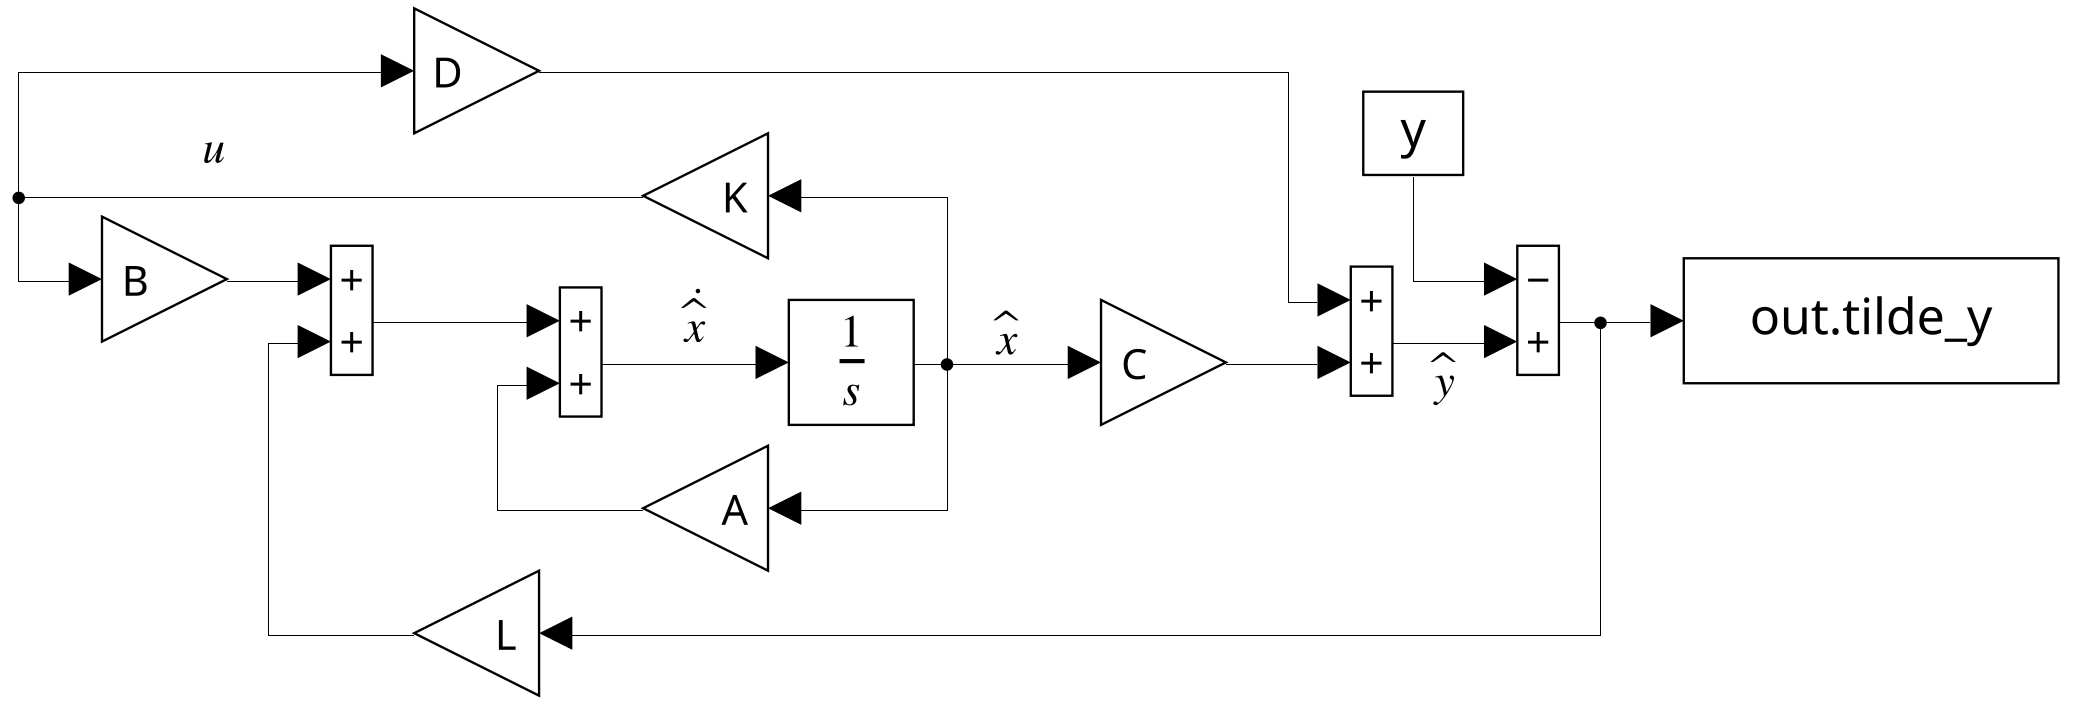
\includegraphics[width=0.9\textwidth]{../images/task3/model3.png}
	\caption{Структурная схема замкнутой системы}
\end{figure}




\subsection{Выбор спектров}


Задамся следующими спектрами:

\[
\sigma(A + BK) = \{-3,\ -3 \pm 4i,\ -5\}
\qquad
\sigma(A + LC) = \{-12,\ -5, -10, -15\}
\]

Все числа лежат в левой полуплоскости --- замкнутая система асимптотически устойчива. Спектр наблюдателя содержит ненаблюдаемое $\lambda_1 = -12$,
а его вещественные части по модулю вдвое больше, чем у регулятора~---
наблюдатель сходится быстрее, чем регулятор успевает среагировать.

\subsection{Синтез регулятора \(K\)}

Синтезирую матрицу $K$ по формуле Басса-Гура:
\[
K = -\bar{a}\, A_a^{-1}\, U^{-1}
\]

Запишу желаемый характеристический полином:
\[
D^*(\lambda) = (\lambda + 3)(\lambda + 3 - 4i)(\lambda + 3 + 4i)(\lambda + 5)
= \lambda^4 + 14\lambda^3 + 88\lambda^2 + 290\lambda + 375
\]

Характеристический полином матрицы $A$:
\[
D(\lambda) = \lambda^4 - 20\lambda^3 - 112\lambda^2 + 2624\lambda - 7680
\]

Матрица разности коэффициентов $\bar{a}$:
\[
\bar{a} = \begin{bmatrix}
	14 - (-20) & 88 - (-112) & 290 - 2624 & 375 - (-7680)
\end{bmatrix}
= \begin{bmatrix}
	34 & 200 & -2334 & 8055
\end{bmatrix}
\]

Матрица $A_a$ из коэффициентов $D(\lambda)$:
\[
A_a = \begin{bmatrix}
	1 & -20 & -112 &  2624 \\
	0 &   1 &  -20 &  -112 \\
	0 &   0 &    1 &   -20 \\
	0 &   0 &    0 &     1
\end{bmatrix}
\]

Матрица управляемости $U_c = \begin{bmatrix} B & AB & A^2B & A^3B \end{bmatrix}$ (листинг~\ref{lst:K3}):

\[
U_c =
\begin{bmatrix}
	3 & -16 & -160 & -9088 \\
	3 &   8 &  512 &  5888 \\
	1 &   8 &  576 &  6656 \\
	3 &  48 &  352 & 10368
\end{bmatrix}
\]

Вычислю $K$ программно (листинг~\ref{lst:K3}):

\[
K = \begin{bmatrix}
	17.50 & -18.20 & -7.00 & -8.30
\end{bmatrix}
\]

Проверю корректность расчётов (листинг~\ref{lst:eig3check}):

\[
A + B K = \begin{bmatrix}
	57.51 & -63.61 & -28 & -23.9 \\
	43.51 & -49.61 & -22 & -17.9 \\
	10.5 & -19.2 &  -2 &   0.7 \\
	53.51 & -47.61 & -12 & -19.9
\end{bmatrix}
\qquad \Longrightarrow \qquad
\sigma(A + BK) = \{-5,\ -3,\ -3 \pm 4i\}
\]

Спектр совпадает с желаемым, матрица регулятора $K$ синтезирована корректно.

\subsection{Синтез матрицы наблюдателя \(L\)}

Столбец $\tilde{C}$, соответствующий $\lambda_1 = -12$, нулевой --- эта мода ненаблюдаема.
Исключу её и составлю усечённую систему из трёх наблюдаемых мод (листинг~\ref{lst:L3}):
\[
\begin{array}{c}
	\begin{array}{cc}
		\tilde{A} =
		\begin{bNiceMatrix}[create-medium-nodes,left-margin=4pt,right-margin=4pt]
			-12 & 0 & 0 & 0 \\
			0 & 4 & 0 & 0 \\
			0 & 0 & 8 & 0 \\
			0 & 0 & 0 & 20 \\
			\CodeAfter
			\tikz \draw[red!80!black,line width=0.7pt,opacity=0.4]
			([xshift=-2pt]1-1-medium.west) -- ([xshift=2pt]1-4-medium.east);
			\tikz \draw[red!80!black,line width=0.7pt,opacity=0.4]
			([yshift=2pt]1-1-medium.north) -- ([yshift=-2pt]4-1-medium.south);
		\end{bNiceMatrix} \\[28pt]
		\tilde{C} =
		\begin{bNiceMatrix}[create-medium-nodes,left-margin=4pt,right-margin=4pt]
			0 & 0 & 4 & 0 \\
			0 & -2 & 0 & 6 \\
			\CodeAfter
			\tikz \draw[red!80!black,line width=0.7pt,opacity=0.4]
			([yshift=2pt]1-1-medium.north) -- ([yshift=-2pt]2-1-medium.south);
		\end{bNiceMatrix}
	\end{array}
	\quad \Longrightarrow \quad
	\begin{array}{cc}
		\tilde{A_c} =
		\begin{bmatrix}
			4 & 0 & 0 \\
			0 & 8 & 0 \\
			0 & 0 & 20
		\end{bmatrix} \\[28pt]
		\tilde{C_c} =
		\begin{bmatrix}
			0 & 4 & 0 \\
			-2 & 0 & 6
		\end{bmatrix}
	\end{array}
\end{array}
\]

Синтезирую $\tilde L_c$ для усечённой системы, после чего дополню нулевой строкой для ненаблюдаемой моды
и перейду в исходный базис:
\[
\tilde{L} =
\begin{bmatrix}
	0 & 0 \\
	\multicolumn{2}{c}{L_c}
\end{bmatrix}
\qquad
L = V\tilde{L}
\]

В результате получаю (листинг~\ref{lst:L3}):
\[
L =
\begin{bmatrix}
	1.25 & -3.06 \\
	-1.25 &  1.97 \\
	1.25 &  3.06 \\
	1.25 &  1.97
\end{bmatrix}
\]

Проверю корректность (листинг~\ref{lst:eigL3}):
\[
\sigma(A + LC) = \{-12,\ -5,\ -10,\ -15\}
\]

Спектр совпадает с желаемым, матрица $L$ синтезирована корректно.\\

В ходе компьютерного моделирования замкнутой системы с наблюдателем я построила графики вектора состояния $x(t)$ и его оценки $\hat{x}(t)$, ошибки наблюдателя $e(t) = x(t) - \hat{x}(t)$, управляющего воздействия $u(t)$ и выхода системы $y(t)$.

\begin{figure}[H]
	\centering
	
\includegraphics[width=0.9\textwidth]{../images/task3/u.pdf}
	\caption{Управляющее воздействие $u(t)$}
\end{figure}
\begin{figure}[H]
	\centering
	
\includegraphics[width=0.9\textwidth]{../images/task3/y.pdf}
	\caption{Выход системы $y(t)$}
\end{figure}
\begin{figure}[H]
	\centering
	\begin{subfigure}[b]{0.45\textwidth}
		\centering
		
\includegraphics[width=\textwidth]{../images/task3/x.pdf}
		\caption{Вектор состояния $x(t)$ и $\hat{x}(t)$}
	\end{subfigure}
	\hfill
	\begin{subfigure}[b]{0.45\textwidth}
		\centering
		
\includegraphics[width=\textwidth]{../images/task3/e.pdf}
		\caption{Ошибка наблюдения $e(t) = x(t) - \hat{x}(t)$}
	\end{subfigure}
	\caption{Результаты моделирования}
\end{figure}

Все компоненты вектора состояния асимптотически сходятся к нулю, что подтверждает корректность синтеза регулятора $K$. Наблюдатель успешно восстанавливает вектор состояния системы --- ошибка $e(t)$ стремится к нулю, то есть $\hat{x}(t) \to x(t)$. Управляющее воздействие $u(t) = K\hat{x}(t)$ также стремится к нулю.




\newpage \subsection{Вывод по заданию}

В задании я синтезировала регулятор $K$ и матрицу коррекции наблюдателя
$L$ для системы с $\sigma(A) = \{-12,\, 4,\, 8,\, 20\}$.
Система полностью управляема; собственное число $\lambda_1 = -12$
ненаблюдаемо, но система обнаруживаема.

По результатам моделирования $x(t) \to 0$, $e(t) \to 0$, $u(t) \to 0$,
что подтверждает корректность синтеза.




\newpage
\section{Наблюдатель пониженного порядка}
\label{sec:task4}


В соответствии с вариантом рассмотрю систему, где матрицы $A$,
$B$, $D$ взяты из Задания~3, а матрица $C$:
\[
C = \begin{bmatrix}
	0 & 1 & 0 & 0 \\
	0 & 0 & 1 & 0
\end{bmatrix}
\]

Требуется:
\begin{itemize}
	\item Найти собственные числа матрицы $A$, определить управляемость
	и наблюдаемость каждого из них.
	\item Построить схему моделирования системы, замкнутой наблюдателем
	пониженного порядка и законом управления $u = K\hat{x}$,
	где $K$ --- регулятор из Задания~\ref{sec:task3}.
	\item Задаться желаемым спектром матрицы $\Gamma$, обеспечивающим
	асимптотическую устойчивость замкнутой системы.
	\item Синтезировать матрицу преобразования $Q$.
	\item Выполнить моделирование при $x(0) = \begin{bmatrix}1&1&1&1
	\end{bmatrix}^{\top}$, $\hat{z}(0) = \begin{bmatrix}0&0
	\end{bmatrix}^{\top}$, построить графики $u(t)$, $\hat{z}(t)$,
	$x(t)$, $\hat{x}(t)$ и $e(t) = x(t) - \hat{x}(t)$.
\end{itemize}

\hrule \newpage


\subsection{Анализ системы}

Поскольку матрицы $A$ и $B$ совпадают с использованными в Задании~\ref{sec:task3},
воспользуюсь результатами анализа управляемости оттуда.
Все собственные числа управляемы, система полностью управляема и стабилизируема:
$$\sigma(A) = \{-12,\, 4,\, 8,\, 20\}$$

Для оценки наблюдаемости каждого собственного числа при новой матрице:
$$C = \begin{bmatrix}
	0 & 1 & 0 & 0 \\
	0 & 0 & 1 & 0
\end{bmatrix}$$
переведу систему в жорданов базис (листинг~\ref{lst:jordan4}):
$$\tilde{C} = C \cdot V =
\begin{bmatrix}
	0.5 & 0.5 & -0.5 & -0.5 \\
	0.5 & -0.5 & 0.5 & -0.5
\end{bmatrix}$$

Все столбцы матрицы $\tilde{C}$ ненулевые, следовательно, все собственные числа
наблюдаемы, система полностью наблюдаема и, следовательно, обнаруживаема.

\subsection{Схема моделирования системы}

Построю модель замкнутой системы:

\begin{figure}[H]
	\centering
	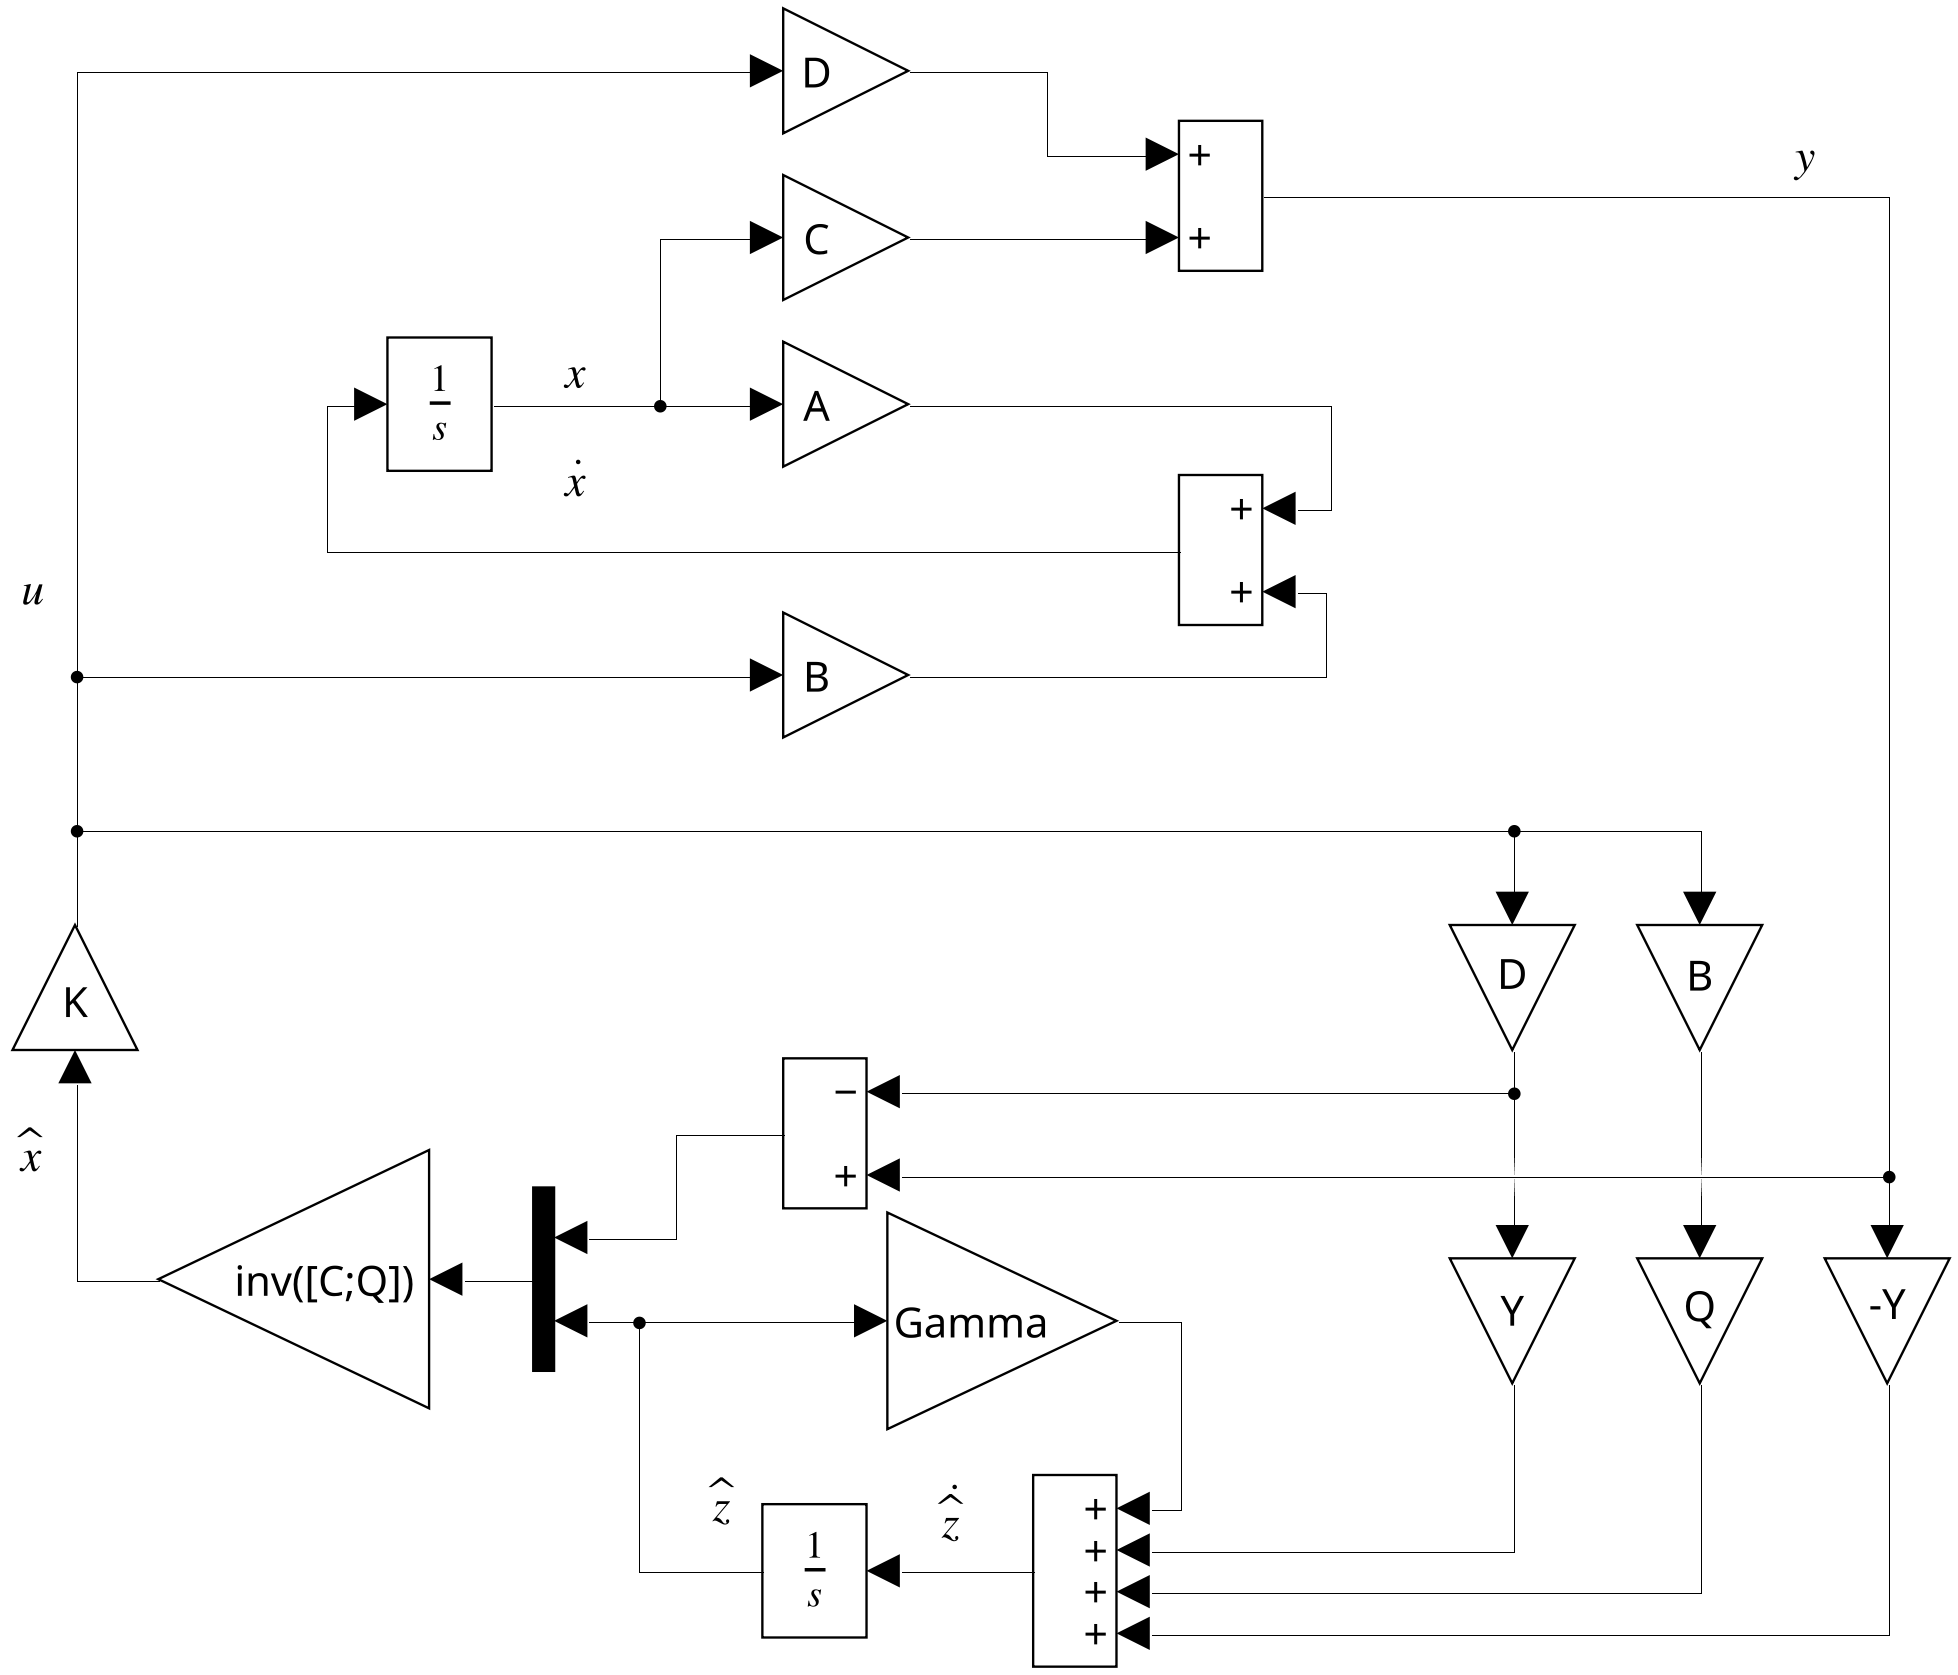
\includegraphics[width=0.9\textwidth]{../images/task4/model4.png}
	\caption{Структурная схема системы}
\end{figure}


\[
\begin{cases}
	
	\dot{x} = Ax + Bu \\[6pt]
	
	y = Cx + Du \\[10pt]
	
	\dot{\hat z} = \Gamma \hat z - Yy + (QB + YD)u \\[10pt]
	
	\hat{x} =
	\begin{bmatrix}
		C \\
		Q
	\end{bmatrix}^{-1}
	\begin{bmatrix}
		y - Du \\
		\hat z
	\end{bmatrix} \\[12pt]
	
	u = K\hat{x}
	
\end{cases}
\]

\subsection{Синтез матрицы преобразования \(Q\)}

Для синтеза матрицы $Q$ воспользуюсь уравнением Сильвестра:
\[
QA - \Gamma Q = YC
\]
где $Y$ --- вспомогательная матрица, выбираемая из условия невырожденности
матрицы $\begin{bmatrix} C \\ Q \end{bmatrix}$.

Выберу матрицу $Y$:
\[
Y = \begin{bmatrix} 3 & 2 \\ 1 & 4 \end{bmatrix}
\]

Решая уравнение Сильвестра программно (листинг~\ref{lst:Q4}),
получаю матрицу преобразования
\[
Q =
\begin{bmatrix}
	-0.6627 & -0.5516 & -0.6151 & 0.6706 \\
	0.3741 & 0.3803 & 0.5245 & -0.3878
\end{bmatrix}
\]

Проверю невырожденность матрицы
\(\begin{bmatrix}
	C \\
	Q
\end{bmatrix}
\)

\[
\det
\begin{bmatrix}
	C \\
	Q
\end{bmatrix}
= 0.0061 \neq 0
\]

Следовательно, условие существования наблюдателя
пониженного порядка выполняется.

\subsection{Компьютерное моделирование}

Выполню компьютерное моделирование системы при начальных условиях
\[
x(0) = 
\begin{bmatrix}
	1 & 1 & 1 & 1
\end{bmatrix}^{\!\top}
\qquad
\hat z(0) =
\begin{bmatrix}
	0 & 0
\end{bmatrix}^{\!\top}
\]

На рис.~\ref{fig:u4} показан сигнал управления $u(t)$, формируемый
модальным регулятором.

\begin{figure}[H]
	\centering
	
\includegraphics[width=0.85\linewidth]{../../report/images/task4/u.pdf}
	\caption{Сигнал управления $u(t)$}
	\label{fig:u4}
\end{figure}

На рис.~\ref{fig:z4} показана динамика состояния наблюдателя
пониженного порядка $\hat z(t)$.

\begin{figure}[H]
	\centering
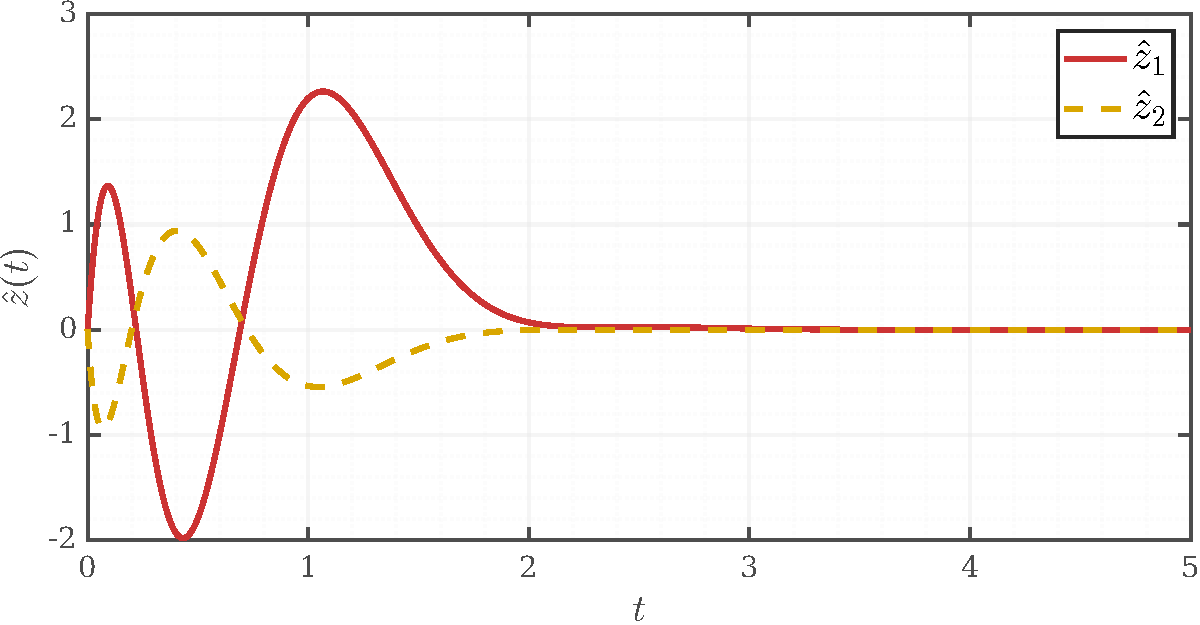
\includegraphics[width=0.85\linewidth]{../../report/images/task4/z.pdf}
\caption{Состояние наблюдателя пониженного порядка $\hat z(t)$}
\label{fig:z4}
\end{figure}

На рис.~\ref{fig:xcmp4} приведены сравнительные графики истинных
состояний системы $x(t)$ и их оценок $\hat x(t)$, формируемых
наблюдателем.

\begin{figure}[H]
\centering
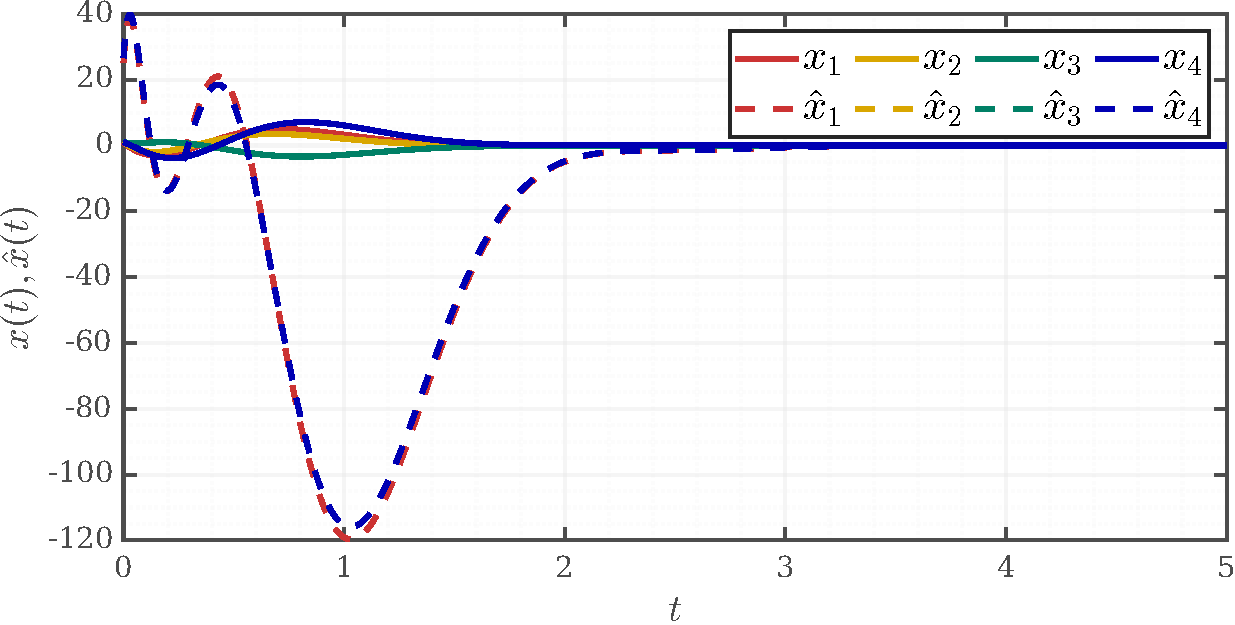
\includegraphics[width=0.85\linewidth]{../../report/images/task4/x_compare.pdf}
\caption{Сравнение состояний $x(t)$ и оценок $\hat x(t)$}
\label{fig:xcmp4}
\end{figure}

На рис.~\ref{fig:e4} показана ошибка наблюдения
\[
e(t) = x(t) - \hat x(t)
\]

\begin{figure}[H]
\centering

\includegraphics[width=0.85\linewidth]{../../report/images/task4/e.pdf}
\caption{Ошибка наблюдателя $e(t)$}
\label{fig:e4}
\end{figure}

Из представленных графиков видно, что состояния системы $x(t)$
асимптотически стремятся к нулю. Оценки состояний $\hat x(t)$,
формируемые наблюдателем пониженного порядка, сходятся к состояниям системы $x(t)$. Ошибка наблюдения $e(t)$ стремится к
нулю, что подтверждает корректность синтеза наблюдателя.

\newpage
\subsection{Вывод по заданию}

В этом задании я синтезировала наблюдатель пониженного порядка и нашла матрицу преобразования $Q$. 
Проверка показала, что матрица $\begin{bmatrix} C \\ Q \end{bmatrix}$ невырождена, поэтому наблюдатель существует.

По результатам моделирования видно, что оценки состояний $\hat{x}(t)$ сходятся к истинным состояниям $x(t)$, 
а ошибка наблюдения стремится к нулю. Это подтверждает корректность синтеза наблюдателя.







\newpage
\section{Вывод}

В ходе работы я исследовала методы синтеза модальных регуляторов и наблюдателей состояния. 
Были рассмотрены модальный регулятор, наблюдатель полного порядка, управление по выходу и 
наблюдатель пониженного порядка.

Для заданной системы были синтезированы матрицы регулятора и наблюдателей, а также 
проведено компьютерное моделирование. По результатам моделирования видно, что состояния 
системы сходятся к нулю, оценки состояний сходятся к состояниям системы, а ошибка наблюдения 
стремится к нулю.

Материалы работы: \href{https://github.com/decadeos/ITMO/tree/master/3_course/TAU/lab2}{\texttt{github.com}}








\newpage
\section{Приложение}

\subsection*{Задание 1}

\begin{lstlisting}[caption={Инициализация}]
A = [8  1  11,
	 4  0  4 ,
	-4 -3  -7,];

B = [-1; -3; 3];
\end{lstlisting}

\begin{lstlisting}[caption={Поиск вещественной Жордановой формы}, label={lst:jordan1}]
[P, J] = jordan(sym(A)); P = double(P); J = double(J);
[P_real, J_real] = cdf2rdf(P, J)
B_tilde = inv(P_real) * B
\end{lstlisting}

\begin{lstlisting}[caption={Решение уравнения Сильвестра}, label={lst:silv1}]
A2 = J_real(2:3, 2:3);
B2 = B_tilde(2:3);
G = [-3 1; 0 -3];
Y = [1 2];

P = lyap(A2, -G, -B2*Y)
K2 = -Y * P^-1
\end{lstlisting}

\begin{lstlisting}[caption={Перевод \(\hat K_c\) в исходный базис}, label={lst:origK11}]
K = [0 K2] * P_real^-1
\end{lstlisting}

\begin{lstlisting}[caption={Собственные числа матрицы замкнутой системы}, label={lst:eig1}]
z = A + B*K
eig(z)
\end{lstlisting}

\begin{lstlisting}[caption={Расчет матрицы \(P_\text{упр}\)}, label={lst:P1}]
Uc = ctrb(A2, B2);
a = poly(A2);
A_up = [ 0 1; -a(3) -a(2) ];
B_up = [0;1];
K_up = [-8992 -334];
Uc_star = ctrb(A_up, B_up);
P_up = Uc_star / Uc
K2 = K_up * P_up
\end{lstlisting}

\begin{lstlisting}[caption={Расчет \(\hat K_c\) методом Басса-Гура\(/\)Акакермана}, label={lst:bassa}]
D_star = [1, 6, 90];   
a_bar = D_star(2:end) - a(2:end);  
Aa = [1, a(2); 0,  1];  
K2 = -a_bar * inv(Aa) * inv(Uc);
\end{lstlisting}

\newpage
\subsection*{Задание 2}

\begin{lstlisting}[caption={Инициализация}]
A = [-40  16   9   7;
	 -64  25  14  12;
	 -26  11   7   3;
	 -48  18  14   8];
C = [-3  2  -2  1];
\end{lstlisting}

\begin{lstlisting}[caption={Собственные числа матрицы системы}, label={lst:eig2}]
eig(A)
\end{lstlisting}

\begin{lstlisting}[caption={Поиск вещественной Жордановой формы}, label={lst:jordan2}]
[P, J] = jordan(sym(A)); P = double(P); J = double(J);
[P_real, J_real] = cdf2rdf(P, J)
C_tilde = C *inv(P_real)
\end{lstlisting}

\begin{lstlisting}[caption={Каноническая форма системы}, label={lst:kanon2}]
a = double(poly(A));
A_k = [0, 0, 0, -a(5);
	   1, 0, 0, -a(4);
	   0, 1, 0, -a(3);
	   0, 0, 1, -a(2);];

C_k = [0, 0, 0, 1;];
\end{lstlisting}

\begin{lstlisting}[caption={Синтез матрицы $L_k$}, label={lst:lk}]
syms l1 l2 l3 l4
L_k = [l1; l2; l3; l4];
eq = A_k + L_k * C_k == Gamma;
sol = solve(eq, [l1 l2 l3 l4]);
L_k = double([sol.l1; sol.l2; sol.l3; sol.l4])
\end{lstlisting}

\begin{lstlisting}[caption={Переход в исходный базис}, label={lst:lobs}]
T = obsv(A_k, C_k) \ obsv(A, C);
L = inv(T) * L_k;
\end{lstlisting}

\begin{lstlisting}[caption={Проверка собственных чисел матрицы замкнутой системы}, label={lst:check}]
z = A + L*C
eig(z)

\end{lstlisting}



\newpage
\subsection*{Задание 3}

\begin{lstlisting}[caption={Инициализация}]
A = [ 5  -9  -7   1;
	 -9   5  -1   7;
	 -7  -1   5   9;
	  1   7   9   5];

B = [3; 3; 1; 3];

C = [ 2  -2   2   2;
-2   4   2   4];

D = [4; 1];
\end{lstlisting}

\begin{lstlisting}[caption={Собственные числа матрицы системы}, label={lst:eig3}]
eig(A)
\end{lstlisting}

\begin{lstlisting}[caption={Поиск вещественной Жордановой формы}, label={lst:jordan3}]
[P, J] = jordan(sym(A)); P = double(P); J = double(J);
[P_real, J_real] = cdf2rdf(P, J)
B_tilde = inv(P_real) * B
C_tilde = C * P_real
\end{lstlisting}

\begin{lstlisting}[caption={Синтез матрицы $K$ методом Басса-Гура}, label={lst:K3}]
D_star = [1, 14, 88, 290, 375];
a = poly(A);
a_bar = D_star(2:end) - a(2:end);

Aa = [1,    a(2), a(3), a(4);
	  0,    1,    a(2), a(3);
      0,    0,    1,    a(2);
	  0,    0,    0,    1  ];

Uc = ctrb(A, B);
K = -a_bar * inv(Aa) * inv(Uc);
\end{lstlisting}

\begin{lstlisting}[caption={Проверка спектра замкнутой системы}, label={lst:eig3check}]
z = A + B*K
eig(z)
\end{lstlisting}

\begin{lstlisting}[caption={Синтез матрицы $L$}, label={lst:L3}]
[V, Lambda] = eig(A);
A_tilde = inv(V) * A * V;
C_tilde = C * V;

[~, idx] = min(vecnorm(C_tilde));
obs_idx = setdiff(1:4, idx);

A_c = diag(diag(Lambda(obs_idx, obs_idx)));
C_c = C_tilde(:, obs_idx);

desired_poles = [-5, -10, -15];
L_c = -place(A_c', C_c', desired_poles)';

L_tilde = zeros(4, 2);
L_tilde(obs_idx, :) = L_c;
L = V * L_tilde
\end{lstlisting}

\begin{lstlisting}[caption={Проверка спектра наблюдателя}, label={lst:eigL3}]
eig(A + L*C)
\end{lstlisting}

\newpage
\subsection*{Задание 4}

\begin{lstlisting}[caption={Инициализация}]
A = [5 -9 -7 1;
	-9  5 -1 7;
	-7 -1  5 9;
	 1  7  9 5];

B = [3; 3; 1; 3];

C = [0 1 0 0;
     0 0 1 0];

D = [4; 1];

\end{lstlisting}

\begin{lstlisting}[caption={Матрица \(C\) в жордане}, label={lst:jordan4}]
[V, Lambda] = eig(A);
C_tilde = C * V
\end{lstlisting}

\begin{lstlisting}[caption={Синтез матрицы $Q$}, label={lst:Q4}]
Gamma = diag([-10, -15]);
Y = [3 2; 1 4];
Q = lyap(-Gamma, A, -Y*C);
det([C;Q])
\end{lstlisting}

\end{document}